\chapter{Range-Rename}
\label{chap:rename}

This chapter describes the range-rename operation on \bets that makes
efficient renames possible on full-path-indexed \betrfs.
To perform a file system rename, \betrfs simply invokes the range-rename
operation on \bets,
which updates all related key/value pairs in an I/O-efficient way.

We first describe the range-rename interface and how \betrfs can use it to
implement file system renames.
Then, we discuss two key techniques that enable efficient range-rename
on \bets, \textbf{tree surgery} and \textbf{key lifting}.
At last, we talk about some implementation details of \betrfs and range-rename.

\section{The range-rename interface}

Range-rename is a new key/value store operation defined as
range-rename(\spre, \dpre).
Define a source key/value pair as a key/value pair whose key has the prefix \spre
and a destination key/value pair as a key/value pair whose key has the prefix \dpre.
Range-rename(\spre, \dpre) does three things:
\begin{itemize}
\item it deletes all destination key/value pairs from the key/value store;
\item then, for any source key/value pair $(k,v)$ in the key/value store,
it inserts a key/value pair $(k',v)$ to the key/value store,
where $k$ is the concatenation of \spre and some suffix $s$ and $k'$ is the
concatenation of \dpre and the same suffix $s$;
\item at last, it deletes all source key/value pairs from the key/value store.
\end{itemize}
In other words, the range-rename deletes all destination key/value pairs and
updates all source key/value pairs to have \dpre.

To see how range-rename accomplishes file system renames in full-path-indexed
\betrfs, consider renaming file ``/foo'' to ``/bar''.
In \mdb, \betrfs needs to insert the destination key ``/bar''
(this insert overwrites the old value of ``/bar'', if it exists)
and delete the source key ``/foo'', resulting in two operations on the \bet.
On the other hand, in \ddb, \betrfs needs to delete all data keys of ``/bar''
(POSIX allows file renames to overwrite the destination file) and update all
data keys of ``/foo'' to be data keys of ``/bar''.
The whole work in \ddb can be done by calling range-rename(``/foo'',``/bar'')
(a data key is the concatenation of the full-path and an 8-byte block number).

Similarly, consider renaming directory ``/baz'' to ``/qux''.
In \mdb, \betrfs also needs to insert the destination key ``/qux'' and delete
the source key ``/baz'' with two operations on the \bet.
Additionally, \betrfs needs to update all keys with prefix ``/baz/'' to have
prefix ``/qux/''
(POSIX only allows directory renames to overwrite an empty directory, which
means there cannot be any key with prefix ``/qux/''),
which is covered in range-rename(``/baz/'', ``/qux/'').
Likewise, in \ddb, \betrfs needs to update all keys with prefix ``/baz/''
to have prefix ``/qux/'', which is done by range-rename(``/baz/'', ``/qux/'')
(directory doesn't have any data key).

\begin{table}[t]
    \centering
    \begin{tabular}{c | l}
        \hline
        Type of Rename & Key/Value Store Operations \\
        \hline
        \hline
        File Rename & \mdb$\rightarrow$put(\textit{dst}); \\
                    & \mdb$\rightarrow$del(\textit{src}); \\
                    & \ddb$\rightarrow$range-rename(\textit{src}, \textit{dst}); \\
        \hline
        Directory Rename & \mdb$\rightarrow$put(\textit{dst}); \\
                         & \mdb$\rightarrow$del(\textit{src}); \\
                         & \mdb$\rightarrow$range-rename(\textit{src/}, \textit{dst/}); \\
                         & \ddb$\rightarrow$range-rename(\textit{src/}, \textit{dst/}); \\
        \hline
    \end{tabular}
    \caption[Full-path-indexed \betrfs implements file system renames with range-rename]{\label{tab:fsrr}
        Full-path-indexed \betrfs renames \textit{src} to \textit{dst} by
        invoking range-rename and other operations on \bets.}
\end{table}

Table~\ref{tab:fsrr} summarizes how file system renames can be done with
range-rename operations in full-path-index \betrfs.
Briefly speaking, full-path-indexed \betrfs can finish a file rename by
invoking three operations on \bets: an insert, a delete and a range-rename.
And a directory rename can be done with an insert, a delete and two
range-renames.
Therefore, efficient renames are possible in full-path-indexed \betrfs if
the \bet can complete the range-rename operation efficiently.

\section{The range-rename operation}

This section describes the approach to do range-rename on the \bet
with a bounded number of IOs.
The efficient range-rename requires lexicographic key order so that keys with
the same prefix are contiguous in the key space.
With contiguous keys, it is possible to have an isolated subtree that contains
and only contains all keys of a certain prefix.
The range-rename performs \textbf{tree surgery} to slice out such isolated
subtrees, which are then moved to other locations on the \bet.
The prefixes of keys in the subtrees are updated automatically through
\textbf{key lifting}, which transforms \bets to lifted \bets.

This section first describes tree surgery and key lifting, and then shows how
range-rename can be done efficiently with these two techniques.

\subsection{Tree surgery}

\begin{figure}
    \begin{subfigure}{\textwidth}
        \centering
        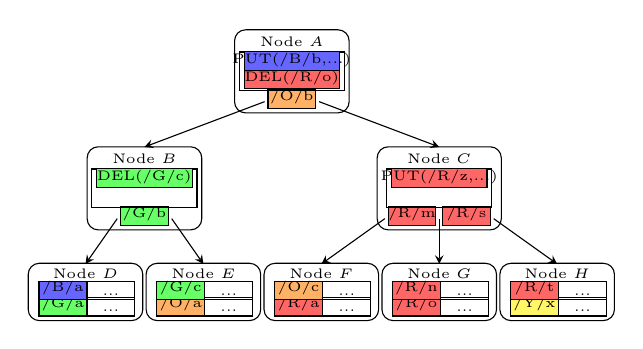
\begin{tikzpicture}[xscale=0.95, yscale=0.95]
            \node[anchor=south, rectangle, rounded corners, minimum height=.06\textwidth, minimum width=.12\textwidth, draw=black] at (0, 0) {};
            \node[anchor=south, font=\tiny] at (0, .036\textwidth) {Node $F$};
            \node[anchor=south, rectangle, minimum height=.015\textwidth, minimum width=.05\textwidth, draw=black, fill={red!60}] at (-.025\textwidth, .005\textwidth) {};
            \node[anchor=south, font=\tiny] at (-.025\textwidth, 0) {/R/a};
            \node[anchor=south, rectangle, minimum height=.015\textwidth, minimum width=.05\textwidth, draw=black] at (.028\textwidth, .005\textwidth) {};
            \node[anchor=south, font=\tiny] at (.028\textwidth, 0) {...};
            \node[anchor=south, rectangle, minimum height=.015\textwidth, minimum width=.05\textwidth, draw=black, fill={orange!60}] at (-.025\textwidth, .023\textwidth) {};
            \node[anchor=south, font=\tiny] at (-.025\textwidth, .018\textwidth) {/O/c};
            \node[anchor=south, rectangle, minimum height=.015\textwidth, minimum width=.05\textwidth, draw=black] at (.028\textwidth, .023\textwidth) {};
            \node[anchor=south, font=\tiny] at (.028\textwidth, .018\textwidth) {...};

            \node[anchor=south, rectangle, rounded corners, minimum height=.06\textwidth, minimum width=.12\textwidth, draw=black] at (.13\textwidth, 0) {};
            \node[anchor=south, font=\tiny] at (.13\textwidth, .036\textwidth) {Node $G$};
            \node[anchor=south, rectangle, minimum height=.015\textwidth, minimum width=.05\textwidth, draw=black, fill={red!60}] at (.105\textwidth, .005\textwidth) {};
            \node[anchor=south, font=\tiny] at (.105\textwidth, 0) {/R/o};
            \node[anchor=south, rectangle, minimum height=.015\textwidth, minimum width=.05\textwidth, draw=black] at (.158\textwidth, .005\textwidth) {};
            \node[anchor=south, font=\tiny] at (.158\textwidth, 0) {...};
            \node[anchor=south, rectangle, minimum height=.015\textwidth, minimum width=.05\textwidth, draw=black, fill={red!60}] at (.105\textwidth, .023\textwidth) {};
            \node[anchor=south, font=\tiny] at (.105\textwidth, .018\textwidth) {/R/n};
            \node[anchor=south, rectangle, minimum height=.015\textwidth, minimum width=.05\textwidth, draw=black] at (.158\textwidth, .023\textwidth) {};
            \node[anchor=south, font=\tiny] at (.158\textwidth, .018\textwidth) {...};

            \node[anchor=south, rectangle, rounded corners, minimum height=.06\textwidth, minimum width=.12\textwidth, draw=black] at (.26\textwidth, 0) {};
            \node[anchor=south, font=\tiny] at (.26\textwidth, .036\textwidth) {Node $H$};
            \node[anchor=south, rectangle, minimum height=.015\textwidth, minimum width=.05\textwidth, draw=black, fill={yellow!60}] at (.235\textwidth, .005\textwidth) {};
            \node[anchor=south, font=\tiny] at (.235\textwidth, 0) {/Y/x};
            \node[anchor=south, rectangle, minimum height=.015\textwidth, minimum width=.05\textwidth, draw=black] at (.288\textwidth, .005\textwidth) {};
            \node[anchor=south, font=\tiny] at (.288\textwidth, 0) {...};
            \node[anchor=south, rectangle, minimum height=.015\textwidth, minimum width=.05\textwidth, draw=black, fill={red!60}] at (.235\textwidth, .023\textwidth) {};
            \node[anchor=south, font=\tiny] at (.235\textwidth, .018\textwidth) {/R/t};
            \node[anchor=south, rectangle, minimum height=.015\textwidth, minimum width=.05\textwidth, draw=black] at (.288\textwidth, .023\textwidth) {};
            \node[anchor=south, font=\tiny] at (.288\textwidth, .018\textwidth) {...};

            \node[anchor=south, rectangle, rounded corners, minimum height=.06\textwidth, minimum width=.12\textwidth, draw=black] at (-.13\textwidth, 0) {};
            \node[anchor=south, font=\tiny] at (-.13\textwidth, .036\textwidth) {Node $E$};
            \node[anchor=south, rectangle, minimum height=.015\textwidth, minimum width=.05\textwidth, draw=black, fill={orange!60}] at (-.155\textwidth, .005\textwidth) {};
            \node[anchor=south, font=\tiny] at (-.155\textwidth, 0) {/O/a};
            \node[anchor=south, rectangle, minimum height=.015\textwidth, minimum width=.05\textwidth, draw=black] at (-.102\textwidth, .005\textwidth) {};
            \node[anchor=south, font=\tiny] at (-.102\textwidth, 0) {...};
            \node[anchor=south, rectangle, minimum height=.015\textwidth, minimum width=.05\textwidth, draw=black, fill={green!60}] at (-.155\textwidth, .023\textwidth) {};
            \node[anchor=south, font=\tiny] at (-.155\textwidth, .018\textwidth) {/G/c};
            \node[anchor=south, rectangle, minimum height=.015\textwidth, minimum width=.05\textwidth, draw=black] at (-.102\textwidth, .023\textwidth) {};
            \node[anchor=south, font=\tiny] at (-.102\textwidth, .018\textwidth) {...};

            \node[anchor=south, rectangle, rounded corners, minimum height=.06\textwidth, minimum width=.12\textwidth, draw=black] at (-.26\textwidth, 0) {};
            \node[anchor=south, font=\tiny] at (-.26\textwidth, .036\textwidth) {Node $D$};
            \node[anchor=south, rectangle, minimum height=.015\textwidth, minimum width=.05\textwidth, draw=black, fill={green!60}] at (-.285\textwidth, .005\textwidth) {};
            \node[anchor=south, font=\tiny] at (-.285\textwidth, 0) {/G/a};
            \node[anchor=south, rectangle, minimum height=.015\textwidth, minimum width=.05\textwidth, draw=black] at (-.232\textwidth, .005\textwidth) {};
            \node[anchor=south, font=\tiny] at (-.232\textwidth, 0) {...};
            \node[anchor=south, rectangle, minimum height=.015\textwidth, minimum width=.05\textwidth, draw=black, fill={blue!60}] at (-.285\textwidth, .023\textwidth) {};
            \node[anchor=south, font=\tiny] at (-.285\textwidth, .018\textwidth) {/B/a};
            \node[anchor=south, rectangle, minimum height=.015\textwidth, minimum width=.05\textwidth, draw=black] at (-.232\textwidth, .023\textwidth) {};
            \node[anchor=south, font=\tiny] at (-.232\textwidth, .018\textwidth) {...};

            \node[anchor=south, rectangle, rounded corners, minimum height=.087\textwidth, minimum width=.12\textwidth, draw=black] at (-.195\textwidth, .1\textwidth) {};
            \node[anchor=south, font=\tiny] at (-.195\textwidth, .163\textwidth) {Node $B$};
            \node[anchor=south, rectangle, minimum height=.015\textwidth, minimum width=.05\textwidth, draw=black, fill={green!60}] at (-.195\textwidth, .105\textwidth) {};
            \node[anchor=south, font=\tiny] at (-.195\textwidth, .1\textwidth) {/G/b};
            \node[anchor=south, rectangle, minimum height=.04\textwidth, minimum width=.11\textwidth, draw=black] at (-.195\textwidth, .125\textwidth) {};
            \node[anchor=south, rectangle, minimum height=.015\textwidth, minimum width=.1\textwidth, draw=black, fill={green!60}] at (-.195\textwidth, .147\textwidth) {};
            \node[anchor=south, font=\tiny] at  (-.195\textwidth, .141\textwidth) {DEL(/G/c)};

            \node[anchor=south, rectangle, rounded corners, minimum height=.087\textwidth, minimum width=.13\textwidth, draw=black] at (.13\textwidth, .1\textwidth) {};
            \node[anchor=south, font=\tiny] at (.13\textwidth, .163\textwidth) {Node $C$};
            \node[anchor=south, rectangle, minimum height=.015\textwidth, minimum width=.05\textwidth, draw=black, fill={red!60}] at (.1\textwidth, .105\textwidth) {};
            \node[anchor=south, font=\tiny] at (.1\textwidth, .1\textwidth) {/R/m};
            \node[anchor=south, rectangle, minimum height=.015\textwidth, minimum width=.05\textwidth, draw=black, fill={red!60}] at (.16\textwidth, .105\textwidth) {};
            \node[anchor=south, font=\tiny] at (.16\textwidth, .1\textwidth) {/R/s};
            \node[anchor=south, rectangle, minimum height=.04\textwidth, minimum width=.11\textwidth, draw=black] at (.13\textwidth, .125\textwidth) {};
            \node[anchor=south, rectangle, minimum height=.015\textwidth, minimum width=.1\textwidth, draw=black, fill={red!60}] at (.13\textwidth, .147\textwidth) {};
            \node[anchor=south, font=\tiny] at  (.13\textwidth, .141\textwidth) {PUT(/R/z,...)};

            \node[anchor=south, rectangle, rounded corners, minimum height=.087\textwidth, minimum width=.12\textwidth, draw=black] at (-.0325\textwidth, .229\textwidth) {};
            \node[anchor=south, font=\tiny] at (-.0325\textwidth, .292\textwidth) {Node $A$};
            \node[anchor=south, rectangle, minimum height=.015\textwidth, minimum width=.05\textwidth, draw=black, fill={orange!60}] at (-.0325\textwidth, .234\textwidth) {};
            \node[anchor=south, font=\tiny] at (-.0325\textwidth, .229\textwidth) {/O/b};
            \node[anchor=south, rectangle, minimum height=.04\textwidth, minimum width=.11\textwidth, draw=black] at (-.0325\textwidth, .254\textwidth) {};
            \node[anchor=south, rectangle, minimum height=.015\textwidth, minimum width=.1\textwidth, draw=black, fill={red!60}] at (-.0325\textwidth, .256\textwidth) {};
            \node[anchor=south, font=\tiny] at  (-.0325\textwidth, .25\textwidth) {DEL(/R/o)};
            \node[anchor=south, rectangle, minimum height=.015\textwidth, minimum width=.1\textwidth, draw=black, fill={blue!60}] at (-.0325\textwidth, .276\textwidth) {};
            \node[anchor=south, font=\tiny] at  (-.0325\textwidth, .27\textwidth) {PUT(/B/b,...)};

            \draw[->, >=stealth] (-.225\textwidth, .113\textwidth) -- (-.26\textwidth, .063\textwidth);
            \draw[->, >=stealth] (-.165\textwidth, .113\textwidth) -- (-.13\textwidth, .063\textwidth);
            \draw[->, >=stealth] (.13\textwidth, .113\textwidth) -- (.13\textwidth, .063\textwidth);
            \draw[->, >=stealth] (.19\textwidth, .113\textwidth) -- (.26\textwidth, .063\textwidth);
            \draw[->, >=stealth] (.07\textwidth, .113\textwidth) -- (0, .063\textwidth);
            \draw[->, >=stealth] (-.0625\textwidth, .242\textwidth) -- (-.195\textwidth, .192\textwidth);
            \draw[->, >=stealth] (-.0025\textwidth, .242\textwidth) -- (.13\textwidth, .192\textwidth);
        \end{tikzpicture}
        \caption{\label{subfig:slice-1} The \bet before tree surgery.}
    \end{subfigure}
    \begin{subfigure}{\textwidth}
        \centering
        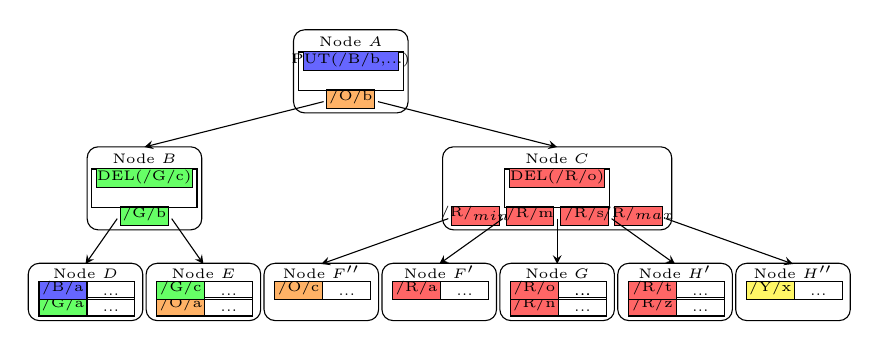
\begin{tikzpicture}[xscale=0.95, yscale=0.95]
            \node[anchor=south, rectangle, rounded corners, minimum height=.06\textwidth, minimum width=.12\textwidth, draw=black] at (0, 0) {};
            \node[anchor=south, font=\tiny] at (0, .036\textwidth) {Node $F''$};
            \node[anchor=south, rectangle, minimum height=.015\textwidth, minimum width=.05\textwidth, draw=black, fill={orange!60}] at (-.025\textwidth, .023\textwidth) {};
            \node[anchor=south, font=\tiny] at (-.025\textwidth, .018\textwidth) {/O/c};
            \node[anchor=south, rectangle, minimum height=.015\textwidth, minimum width=.05\textwidth, draw=black] at (.028\textwidth, .023\textwidth) {};
            \node[anchor=south, font=\tiny] at (.028\textwidth, .018\textwidth) {...};

            \node[anchor=south, rectangle, rounded corners, minimum height=.06\textwidth, minimum width=.12\textwidth, draw=black] at (.13\textwidth, 0) {};
            \node[anchor=south, font=\tiny] at (.13\textwidth, .036\textwidth) {Node $F'$};
            \node[anchor=south, rectangle, minimum height=.015\textwidth, minimum width=.05\textwidth, draw=black, fill={red!60}] at (.105\textwidth, .023\textwidth) {};
            \node[anchor=south, font=\tiny] at (.105\textwidth, .018\textwidth) {/R/a};
            \node[anchor=south, rectangle, minimum height=.015\textwidth, minimum width=.05\textwidth, draw=black] at (.158\textwidth, .023\textwidth) {};
            \node[anchor=south, font=\tiny] at (.158\textwidth, .018\textwidth) {...};

            \node[anchor=south, rectangle, rounded corners, minimum height=.06\textwidth, minimum width=.12\textwidth, draw=black] at (.26\textwidth, 0) {};
            \node[anchor=south, font=\tiny] at (.26\textwidth, .036\textwidth) {Node $G$};
            \node[anchor=south, rectangle, minimum height=.015\textwidth, minimum width=.05\textwidth, draw=black, fill={red!60}] at (.235\textwidth, .005\textwidth) {};
            \node[anchor=south, font=\tiny] at (.235\textwidth, 0) {/R/n};
            \node[anchor=south, rectangle, minimum height=.015\textwidth, minimum width=.05\textwidth, draw=black] at (.288\textwidth, .005\textwidth) {};
            \node[anchor=south, font=\tiny] at (.288\textwidth, 0) {...};
            \node[anchor=south, rectangle, minimum height=.015\textwidth, minimum width=.05\textwidth, draw=black, fill={red!60}] at (.235\textwidth, .023\textwidth) {};
            \node[anchor=south, font=\tiny] at (.235\textwidth, .018\textwidth) {/R/o};
            \node[anchor=south, rectangle, minimum height=.015\textwidth, minimum width=.05\textwidth, draw=black] at (.288\textwidth, .023\textwidth) {};
            \node[anchor=south, font=\tiny] at (.288\textwidth, .018\textwidth) {...};

            \node[anchor=south, rectangle, rounded corners, minimum height=.06\textwidth, minimum width=.12\textwidth, draw=black] at (.39\textwidth, 0) {};
            \node[anchor=south, font=\tiny] at (.39\textwidth, .036\textwidth) {Node $H'$};
            \node[anchor=south, rectangle, minimum height=.015\textwidth, minimum width=.05\textwidth, draw=black, fill={red!60}] at (.365\textwidth, .005\textwidth) {};
            \node[anchor=south, font=\tiny] at (.365\textwidth, 0) {/R/z};
            \node[anchor=south, rectangle, minimum height=.015\textwidth, minimum width=.05\textwidth, draw=black] at (.418\textwidth, .005\textwidth) {};
            \node[anchor=south, font=\tiny] at (.418\textwidth, 0) {...};
            \node[anchor=south, rectangle, minimum height=.015\textwidth, minimum width=.05\textwidth, draw=black, fill={red!60}] at (.365\textwidth, .023\textwidth) {};
            \node[anchor=south, font=\tiny] at (.365\textwidth, .018\textwidth) {/R/t};
            \node[anchor=south, rectangle, minimum height=.015\textwidth, minimum width=.05\textwidth, draw=black] at (.418\textwidth, .023\textwidth) {};
            \node[anchor=south, font=\tiny] at (.418\textwidth, .018\textwidth) {...};

            \node[anchor=south, rectangle, rounded corners, minimum height=.06\textwidth, minimum width=.12\textwidth, draw=black] at (.52\textwidth, 0) {};
            \node[anchor=south, font=\tiny] at (.52\textwidth, .036\textwidth) {Node $H''$};
            \node[anchor=south, rectangle, minimum height=.015\textwidth, minimum width=.05\textwidth, draw=black, fill={yellow!60}] at (.495\textwidth, .023\textwidth) {};
            \node[anchor=south, font=\tiny] at (.495\textwidth, .018\textwidth) {/Y/x};
            \node[anchor=south, rectangle, minimum height=.015\textwidth, minimum width=.05\textwidth, draw=black] at (.548\textwidth, .023\textwidth) {};
            \node[anchor=south, font=\tiny] at (.548\textwidth, .018\textwidth) {...};

            \node[anchor=south, rectangle, minimum height=.015\textwidth, minimum width=.05\textwidth, draw=black] at (.288\textwidth, .023\textwidth) {};
            \node[anchor=south, font=\tiny] at (.288\textwidth, .018\textwidth) {...};
            \node[anchor=south, rectangle, rounded corners, minimum height=.06\textwidth, minimum width=.12\textwidth, draw=black] at (-.13\textwidth, 0) {};
            \node[anchor=south, font=\tiny] at (-.13\textwidth, .036\textwidth) {Node $E$};
            \node[anchor=south, rectangle, minimum height=.015\textwidth, minimum width=.05\textwidth, draw=black, fill={orange!60}] at (-.155\textwidth, .005\textwidth) {};
            \node[anchor=south, font=\tiny] at (-.155\textwidth, 0) {/O/a};
            \node[anchor=south, rectangle, minimum height=.015\textwidth, minimum width=.05\textwidth, draw=black] at (-.102\textwidth, .005\textwidth) {};
            \node[anchor=south, font=\tiny] at (-.102\textwidth, 0) {...};
            \node[anchor=south, rectangle, minimum height=.015\textwidth, minimum width=.05\textwidth, draw=black, fill={green!60}] at (-.155\textwidth, .023\textwidth) {};
            \node[anchor=south, font=\tiny] at (-.155\textwidth, .018\textwidth) {/G/c};
            \node[anchor=south, rectangle, minimum height=.015\textwidth, minimum width=.05\textwidth, draw=black] at (-.102\textwidth, .023\textwidth) {};
            \node[anchor=south, font=\tiny] at (-.102\textwidth, .018\textwidth) {...};

            \node[anchor=south, rectangle, rounded corners, minimum height=.06\textwidth, minimum width=.12\textwidth, draw=black] at (-.26\textwidth, 0) {};
            \node[anchor=south, font=\tiny] at (-.26\textwidth, .036\textwidth) {Node $D$};
            \node[anchor=south, rectangle, minimum height=.015\textwidth, minimum width=.05\textwidth, draw=black, fill={green!60}] at (-.285\textwidth, .005\textwidth) {};
            \node[anchor=south, font=\tiny] at (-.285\textwidth, 0) {/G/a};
            \node[anchor=south, rectangle, minimum height=.015\textwidth, minimum width=.05\textwidth, draw=black] at (-.232\textwidth, .005\textwidth) {};
            \node[anchor=south, font=\tiny] at (-.232\textwidth, 0) {...};
            \node[anchor=south, rectangle, minimum height=.015\textwidth, minimum width=.05\textwidth, draw=black, fill={blue!60}] at (-.285\textwidth, .023\textwidth) {};
            \node[anchor=south, font=\tiny] at (-.285\textwidth, .018\textwidth) {/B/a};
            \node[anchor=south, rectangle, minimum height=.015\textwidth, minimum width=.05\textwidth, draw=black] at (-.232\textwidth, .023\textwidth) {};
            \node[anchor=south, font=\tiny] at (-.232\textwidth, .018\textwidth) {...};

            \node[anchor=south, rectangle, rounded corners, minimum height=.087\textwidth, minimum width=.12\textwidth, draw=black] at (-.195\textwidth, .1\textwidth) {};
            \node[anchor=south, font=\tiny] at (-.195\textwidth, .163\textwidth) {Node $B$};
            \node[anchor=south, rectangle, minimum height=.015\textwidth, minimum width=.05\textwidth, draw=black, fill={green!60}] at (-.195\textwidth, .105\textwidth) {};
            \node[anchor=south, font=\tiny] at (-.195\textwidth, .1\textwidth) {/G/b};
            \node[anchor=south, rectangle, minimum height=.04\textwidth, minimum width=.11\textwidth, draw=black] at (-.195\textwidth, .125\textwidth) {};
            \node[anchor=south, rectangle, minimum height=.015\textwidth, minimum width=.1\textwidth, draw=black, fill={green!60}] at (-.195\textwidth, .147\textwidth) {};
            \node[anchor=south, font=\tiny] at  (-.195\textwidth, .141\textwidth) {DEL(/G/c)};

            \node[anchor=south, rectangle, rounded corners, minimum height=.087\textwidth, minimum width=.24\textwidth, draw=black] at (.26\textwidth, .1\textwidth) {};
            \node[anchor=south, font=\tiny] at (.26\textwidth, .163\textwidth) {Node $C$};
            \node[anchor=south, rectangle, minimum height=.015\textwidth, minimum width=.05\textwidth, draw=black, fill={red!60}] at (.17\textwidth, .105\textwidth) {};
            \node[anchor=south, font=\tiny] at (.17\textwidth, .1\textwidth) {/R/$_{min}$};
            \node[anchor=south, rectangle, minimum height=.015\textwidth, minimum width=.05\textwidth, draw=black, fill={red!60}] at (.23\textwidth, .105\textwidth) {};
            \node[anchor=south, font=\tiny] at (.23\textwidth, .1\textwidth) {/R/m};
            \node[anchor=south, rectangle, minimum height=.015\textwidth, minimum width=.05\textwidth, draw=black, fill={red!60}] at (.29\textwidth, .105\textwidth) {};
            \node[anchor=south, font=\tiny] at (.29\textwidth, .1\textwidth) {/R/s};
            \node[anchor=south, rectangle, minimum height=.015\textwidth, minimum width=.05\textwidth, draw=black, fill={red!60}] at (.35\textwidth, .105\textwidth) {};
            \node[anchor=south, font=\tiny] at (.35\textwidth, .1\textwidth) {/R/$_{max}$};
            \node[anchor=south, rectangle, minimum height=.04\textwidth, minimum width=.11\textwidth, draw=black] at (.26\textwidth, .125\textwidth) {};
            \node[anchor=south, rectangle, minimum height=.015\textwidth, minimum width=.1\textwidth, draw=black, fill={red!60}] at (.26\textwidth, .147\textwidth) {};
            \node[anchor=south, font=\tiny] at  (.26\textwidth, .141\textwidth) {DEL(/R/o)};

            \node[anchor=south, rectangle, rounded corners, minimum height=.087\textwidth, minimum width=.12\textwidth, draw=black] at (.0325\textwidth, .229\textwidth) {};
            \node[anchor=south, font=\tiny] at (.0325\textwidth, .292\textwidth) {Node $A$};
            \node[anchor=south, rectangle, minimum height=.015\textwidth, minimum width=.05\textwidth, draw=black, fill={orange!60}] at (.0325\textwidth, .234\textwidth) {};
            \node[anchor=south, font=\tiny] at (.0325\textwidth, .229\textwidth) {/O/b};
            \node[anchor=south, rectangle, minimum height=.04\textwidth, minimum width=.11\textwidth, draw=black] at (.0325\textwidth, .254\textwidth) {};
            \node[anchor=south, rectangle, minimum height=.015\textwidth, minimum width=.1\textwidth, draw=black, fill={blue!60}] at (.0325\textwidth, .276\textwidth) {};
            \node[anchor=south, font=\tiny] at  (.0325\textwidth, .27\textwidth) {PUT(/B/b,...)};

            \draw[->, >=stealth] (-.225\textwidth, .113\textwidth) -- (-.26\textwidth, .063\textwidth);
            \draw[->, >=stealth] (-.165\textwidth, .113\textwidth) -- (-.13\textwidth, .063\textwidth);
            \draw[->, >=stealth] (.26\textwidth, .113\textwidth) -- (.26\textwidth, .063\textwidth);
            \draw[->, >=stealth] (.32\textwidth, .113\textwidth) -- (.39\textwidth, .063\textwidth);
            \draw[->, >=stealth] (.38\textwidth, .113\textwidth) -- (.52\textwidth, .063\textwidth);
            \draw[->, >=stealth] (.20\textwidth, .113\textwidth) -- (.13\textwidth, .063\textwidth);
            \draw[->, >=stealth] (.14\textwidth, .113\textwidth) -- (0, .063\textwidth);
            \draw[->, >=stealth] (.0025\textwidth, .242\textwidth) -- (-.195\textwidth, .192\textwidth);
            \draw[->, >=stealth] (.0625\textwidth, .242\textwidth) -- (.26\textwidth, .192\textwidth);
        \end{tikzpicture}
        \caption{\label{subfig:slice-2} Tree surgery splits leaf nodes.}
    \end{subfigure}
    \begin{subfigure}{\textwidth}
        \centering
        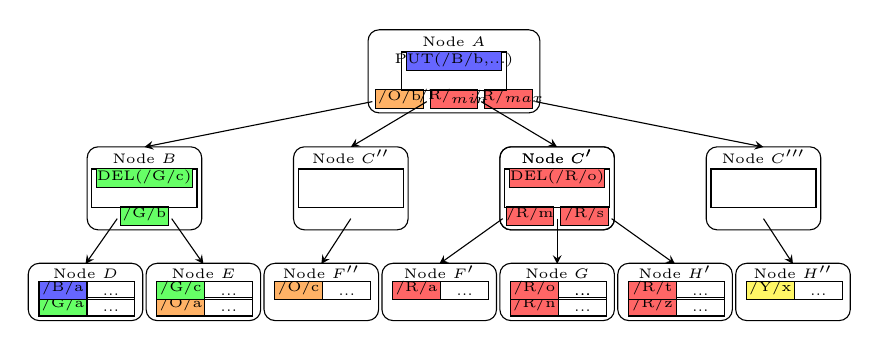
\begin{tikzpicture}[xscale=0.95, yscale=0.95]
            \node[anchor=south, rectangle, rounded corners, minimum height=.06\textwidth, minimum width=.12\textwidth, draw=black] at (0, 0) {};
            \node[anchor=south, font=\tiny] at (0, .036\textwidth) {Node $F''$};
            \node[anchor=south, rectangle, minimum height=.015\textwidth, minimum width=.05\textwidth, draw=black, fill={orange!60}] at (-.025\textwidth, .023\textwidth) {};
            \node[anchor=south, font=\tiny] at (-.025\textwidth, .018\textwidth) {/O/c};
            \node[anchor=south, rectangle, minimum height=.015\textwidth, minimum width=.05\textwidth, draw=black] at (.028\textwidth, .023\textwidth) {};
            \node[anchor=south, font=\tiny] at (.028\textwidth, .018\textwidth) {...};

            \node[anchor=south, rectangle, rounded corners, minimum height=.06\textwidth, minimum width=.12\textwidth, draw=black] at (.13\textwidth, 0) {};
            \node[anchor=south, font=\tiny] at (.13\textwidth, .036\textwidth) {Node $F'$};
            \node[anchor=south, rectangle, minimum height=.015\textwidth, minimum width=.05\textwidth, draw=black, fill={red!60}] at (.105\textwidth, .023\textwidth) {};
            \node[anchor=south, font=\tiny] at (.105\textwidth, .018\textwidth) {/R/a};
            \node[anchor=south, rectangle, minimum height=.015\textwidth, minimum width=.05\textwidth, draw=black] at (.158\textwidth, .023\textwidth) {};
            \node[anchor=south, font=\tiny] at (.158\textwidth, .018\textwidth) {...};

            \node[anchor=south, rectangle, rounded corners, minimum height=.06\textwidth, minimum width=.12\textwidth, draw=black] at (.26\textwidth, 0) {};
            \node[anchor=south, font=\tiny] at (.26\textwidth, .036\textwidth) {Node $G$};
            \node[anchor=south, rectangle, minimum height=.015\textwidth, minimum width=.05\textwidth, draw=black, fill={red!60}] at (.235\textwidth, .005\textwidth) {};
            \node[anchor=south, font=\tiny] at (.235\textwidth, 0) {/R/n};
            \node[anchor=south, rectangle, minimum height=.015\textwidth, minimum width=.05\textwidth, draw=black] at (.288\textwidth, .005\textwidth) {};
            \node[anchor=south, font=\tiny] at (.288\textwidth, 0) {...};
            \node[anchor=south, rectangle, minimum height=.015\textwidth, minimum width=.05\textwidth, draw=black, fill={red!60}] at (.235\textwidth, .023\textwidth) {};
            \node[anchor=south, font=\tiny] at (.235\textwidth, .018\textwidth) {/R/o};
            \node[anchor=south, rectangle, minimum height=.015\textwidth, minimum width=.05\textwidth, draw=black] at (.288\textwidth, .023\textwidth) {};
            \node[anchor=south, font=\tiny] at (.288\textwidth, .018\textwidth) {...};

            \node[anchor=south, rectangle, rounded corners, minimum height=.06\textwidth, minimum width=.12\textwidth, draw=black] at (.39\textwidth, 0) {};
            \node[anchor=south, font=\tiny] at (.39\textwidth, .036\textwidth) {Node $H'$};
            \node[anchor=south, rectangle, minimum height=.015\textwidth, minimum width=.05\textwidth, draw=black, fill={red!60}] at (.365\textwidth, .005\textwidth) {};
            \node[anchor=south, font=\tiny] at (.365\textwidth, 0) {/R/z};
            \node[anchor=south, rectangle, minimum height=.015\textwidth, minimum width=.05\textwidth, draw=black] at (.418\textwidth, .005\textwidth) {};
            \node[anchor=south, font=\tiny] at (.418\textwidth, 0) {...};
            \node[anchor=south, rectangle, minimum height=.015\textwidth, minimum width=.05\textwidth, draw=black, fill={red!60}] at (.365\textwidth, .023\textwidth) {};
            \node[anchor=south, font=\tiny] at (.365\textwidth, .018\textwidth) {/R/t};
            \node[anchor=south, rectangle, minimum height=.015\textwidth, minimum width=.05\textwidth, draw=black] at (.418\textwidth, .023\textwidth) {};
            \node[anchor=south, font=\tiny] at (.418\textwidth, .018\textwidth) {...};

            \node[anchor=south, rectangle, rounded corners, minimum height=.06\textwidth, minimum width=.12\textwidth, draw=black] at (.52\textwidth, 0) {};
            \node[anchor=south, font=\tiny] at (.52\textwidth, .036\textwidth) {Node $H''$};
            \node[anchor=south, rectangle, minimum height=.015\textwidth, minimum width=.05\textwidth, draw=black, fill={yellow!60}] at (.495\textwidth, .023\textwidth) {};
            \node[anchor=south, font=\tiny] at (.495\textwidth, .018\textwidth) {/Y/x};
            \node[anchor=south, rectangle, minimum height=.015\textwidth, minimum width=.05\textwidth, draw=black] at (.548\textwidth, .023\textwidth) {};
            \node[anchor=south, font=\tiny] at (.548\textwidth, .018\textwidth) {...};

            \node[anchor=south, rectangle, minimum height=.015\textwidth, minimum width=.05\textwidth, draw=black] at (.288\textwidth, .023\textwidth) {};
            \node[anchor=south, font=\tiny] at (.288\textwidth, .018\textwidth) {...};
            \node[anchor=south, rectangle, rounded corners, minimum height=.06\textwidth, minimum width=.12\textwidth, draw=black] at (-.13\textwidth, 0) {};
            \node[anchor=south, font=\tiny] at (-.13\textwidth, .036\textwidth) {Node $E$};
            \node[anchor=south, rectangle, minimum height=.015\textwidth, minimum width=.05\textwidth, draw=black, fill={orange!60}] at (-.155\textwidth, .005\textwidth) {};
            \node[anchor=south, font=\tiny] at (-.155\textwidth, 0) {/O/a};
            \node[anchor=south, rectangle, minimum height=.015\textwidth, minimum width=.05\textwidth, draw=black] at (-.102\textwidth, .005\textwidth) {};
            \node[anchor=south, font=\tiny] at (-.102\textwidth, 0) {...};
            \node[anchor=south, rectangle, minimum height=.015\textwidth, minimum width=.05\textwidth, draw=black, fill={green!60}] at (-.155\textwidth, .023\textwidth) {};
            \node[anchor=south, font=\tiny] at (-.155\textwidth, .018\textwidth) {/G/c};
            \node[anchor=south, rectangle, minimum height=.015\textwidth, minimum width=.05\textwidth, draw=black] at (-.102\textwidth, .023\textwidth) {};
            \node[anchor=south, font=\tiny] at (-.102\textwidth, .018\textwidth) {...};

            \node[anchor=south, rectangle, rounded corners, minimum height=.06\textwidth, minimum width=.12\textwidth, draw=black] at (-.26\textwidth, 0) {};
            \node[anchor=south, font=\tiny] at (-.26\textwidth, .036\textwidth) {Node $D$};
            \node[anchor=south, rectangle, minimum height=.015\textwidth, minimum width=.05\textwidth, draw=black, fill={green!60}] at (-.285\textwidth, .005\textwidth) {};
            \node[anchor=south, font=\tiny] at (-.285\textwidth, 0) {/G/a};
            \node[anchor=south, rectangle, minimum height=.015\textwidth, minimum width=.05\textwidth, draw=black] at (-.232\textwidth, .005\textwidth) {};
            \node[anchor=south, font=\tiny] at (-.232\textwidth, 0) {...};
            \node[anchor=south, rectangle, minimum height=.015\textwidth, minimum width=.05\textwidth, draw=black, fill={blue!60}] at (-.285\textwidth, .023\textwidth) {};
            \node[anchor=south, font=\tiny] at (-.285\textwidth, .018\textwidth) {/B/a};
            \node[anchor=south, rectangle, minimum height=.015\textwidth, minimum width=.05\textwidth, draw=black] at (-.232\textwidth, .023\textwidth) {};
            \node[anchor=south, font=\tiny] at (-.232\textwidth, .018\textwidth) {...};

            \node[anchor=south, rectangle, rounded corners, minimum height=.087\textwidth, minimum width=.12\textwidth, draw=black] at (-.195\textwidth, .1\textwidth) {};
            \node[anchor=south, font=\tiny] at (-.195\textwidth, .163\textwidth) {Node $B$};
            \node[anchor=south, rectangle, minimum height=.015\textwidth, minimum width=.05\textwidth, draw=black, fill={green!60}] at (-.195\textwidth, .105\textwidth) {};
            \node[anchor=south, font=\tiny] at (-.195\textwidth, .1\textwidth) {/G/b};
            \node[anchor=south, rectangle, minimum height=.04\textwidth, minimum width=.11\textwidth, draw=black] at (-.195\textwidth, .125\textwidth) {};
            \node[anchor=south, rectangle, minimum height=.015\textwidth, minimum width=.1\textwidth, draw=black, fill={green!60}] at (-.195\textwidth, .147\textwidth) {};
            \node[anchor=south, font=\tiny] at  (-.195\textwidth, .141\textwidth) {DEL(/G/c)};

            \node[anchor=south, rectangle, rounded corners, minimum height=.087\textwidth, minimum width=.12\textwidth, draw=black] at (.0325\textwidth, .1\textwidth) {};
            \node[anchor=south, font=\tiny] at (.0325\textwidth, .163\textwidth) {Node $C''$};
            \node[anchor=south, rectangle, minimum height=.04\textwidth, minimum width=.11\textwidth, draw=black] at (.0325\textwidth, .125\textwidth) {};

            \node[anchor=south, rectangle, rounded corners, minimum height=.087\textwidth, minimum width=.12\textwidth, draw=black] at (.26\textwidth, .1\textwidth) {};
            \node[anchor=south, font=\tiny] at (.26\textwidth, .163\textwidth) {Node $C'$};
            \node[anchor=south, rectangle, minimum height=.015\textwidth, minimum width=.05\textwidth, draw=black, fill={red!60}] at (.23\textwidth, .105\textwidth) {};
            \node[anchor=south, font=\tiny] at (.23\textwidth, .1\textwidth) {/R/m};
            \node[anchor=south, rectangle, minimum height=.015\textwidth, minimum width=.05\textwidth, draw=black, fill={red!60}] at (.29\textwidth, .105\textwidth) {};
            \node[anchor=south, font=\tiny] at (.29\textwidth, .1\textwidth) {/R/s};
            \node[anchor=south, rectangle, minimum height=.04\textwidth, minimum width=.11\textwidth, draw=black] at (.26\textwidth, .125\textwidth) {};
            \node[anchor=south, rectangle, minimum height=.015\textwidth, minimum width=.1\textwidth, draw=black, fill={red!60}] at (.26\textwidth, .147\textwidth) {};
            \node[anchor=south, font=\tiny] at  (.26\textwidth, .141\textwidth) {DEL(/R/o)};

            \node[anchor=south, rectangle, rounded corners, minimum height=.087\textwidth, minimum width=.12\textwidth, draw=black] at (.4875\textwidth, .1\textwidth) {};
            \node[anchor=south, font=\tiny] at (.4875\textwidth, .163\textwidth) {Node $C'''$};
            \node[anchor=south, rectangle, minimum height=.04\textwidth, minimum width=.11\textwidth, draw=black] at (.4875\textwidth, .125\textwidth) {};

            \node[anchor=south, rectangle, rounded corners, minimum height=.087\textwidth, minimum width=.12\textwidth, draw=black] at (.26\textwidth, .1\textwidth) {};
            \node[anchor=south, font=\tiny] at (.26\textwidth, .163\textwidth) {Node $C'$};
            \node[anchor=south, rectangle, minimum height=.015\textwidth, minimum width=.05\textwidth, draw=black, fill={red!60}] at (.23\textwidth, .105\textwidth) {};
            \node[anchor=south, font=\tiny] at (.23\textwidth, .1\textwidth) {/R/m};
            \node[anchor=south, rectangle, minimum height=.015\textwidth, minimum width=.05\textwidth, draw=black, fill={red!60}] at (.29\textwidth, .105\textwidth) {};
            \node[anchor=south, font=\tiny] at (.29\textwidth, .1\textwidth) {/R/s};
            \node[anchor=south, rectangle, minimum height=.04\textwidth, minimum width=.11\textwidth, draw=black] at (.26\textwidth, .125\textwidth) {};
            \node[anchor=south, rectangle, minimum height=.015\textwidth, minimum width=.1\textwidth, draw=black, fill={red!60}] at (.26\textwidth, .147\textwidth) {};
            \node[anchor=south, font=\tiny] at  (.26\textwidth, .141\textwidth) {DEL(/R/o)};

            \node[anchor=south, rectangle, rounded corners, minimum height=.087\textwidth, minimum width=.18\textwidth, draw=black] at (.14625\textwidth, .229\textwidth) {};
            \node[anchor=south, font=\tiny] at (.14625\textwidth, .292\textwidth) {Node $A$};
            \node[anchor=south, rectangle, minimum height=.015\textwidth, minimum width=.05\textwidth, draw=black, fill={orange!60}] at (.08625\textwidth, .234\textwidth) {};
            \node[anchor=south, font=\tiny] at (.08625\textwidth, .229\textwidth) {/O/b};
            \node[anchor=south, rectangle, minimum height=.015\textwidth, minimum width=.05\textwidth, draw=black, fill={red!60}] at (.14625\textwidth, .234\textwidth) {};
            \node[anchor=south, font=\tiny] at (.14625\textwidth, .229\textwidth) {/R/$_{min}$};
            \node[anchor=south, rectangle, minimum height=.015\textwidth, minimum width=.05\textwidth, draw=black, fill={red!60}] at (.20625\textwidth, .234\textwidth) {};
            \node[anchor=south, font=\tiny] at (.20625\textwidth, .229\textwidth) {/R/$_{max}$};
            \node[anchor=south, rectangle, minimum height=.04\textwidth, minimum width=.11\textwidth, draw=black] at (.14625\textwidth, .254\textwidth) {};
            \node[anchor=south, rectangle, minimum height=.015\textwidth, minimum width=.1\textwidth, draw=black, fill={blue!60}] at (.14625\textwidth, .276\textwidth) {};
            \node[anchor=south, font=\tiny] at  (.14625\textwidth, .27\textwidth) {PUT(/B/b,...)};

            \draw[->, >=stealth] (-.225\textwidth, .113\textwidth) -- (-.26\textwidth, .063\textwidth);
            \draw[->, >=stealth] (-.165\textwidth, .113\textwidth) -- (-.13\textwidth, .063\textwidth);
            \draw[->, >=stealth] (.26\textwidth, .113\textwidth) -- (.26\textwidth, .063\textwidth);
            \draw[->, >=stealth] (.32\textwidth, .113\textwidth) -- (.39\textwidth, .063\textwidth);
            \draw[->, >=stealth] (.4875\textwidth, .113\textwidth) -- (.52\textwidth, .063\textwidth);
            \draw[->, >=stealth] (.20\textwidth, .113\textwidth) -- (.13\textwidth, .063\textwidth);
            \draw[->, >=stealth] (.0325\textwidth, .113\textwidth) -- (0, .063\textwidth);
            \draw[->, >=stealth] (.05625\textwidth, .242\textwidth) -- (-.195\textwidth, .192\textwidth);
            \draw[->, >=stealth] (.11625\textwidth, .242\textwidth) -- (.0325\textwidth, .192\textwidth);
            \draw[->, >=stealth] (.17625\textwidth, .242\textwidth) -- (.26\textwidth, .192\textwidth);
            \draw[->, >=stealth] (.23625\textwidth, .242\textwidth) -- (.4875\textwidth, .192\textwidth);
        \end{tikzpicture}
        \caption{\label{subfig:slice-3} Tree surgery splits the LCA.}
    \end{subfigure}
    \caption[Tree surgery example]{\label{fig:slice}
        Tree surgery slices out an isolated subtree of prefix ``/R/''.}
\end{figure}

The goal of tree surgery is to slice out an isolated subtree of a certain
prefix $p$ on the \bet.
In the \bet, each node covers a certain key range, bounded by the key range and
pivots of its parent.
For a certain key range $(p_{min}, p_{max})$ ($p_{min}$ and $p_{max}$ are the
minimum and maximum keys with prefix $p$, respectively), there are three types
of nodes in the \bet:
nodes whose key ranges are completely out of the key range (exterior nodes),
nodes whose key ranges are completely in the key range (interior nodes),
and nodes whose key ranges partly overlap with the key range (fringe nodes).

Figure~\ref{subfig:slice-1} shows an example of a \bet.
Node $A$, $B$ and $C$ are non-leaf nodes with buffers and pivots, while
Node $D$, $E$, $F$, $G$ and $H$ are leaf nodes that only store key/value pairs.
Parent-to-leaf pointers link all nodes into a tree.
Consider prefix ``/R/'',
Node $B$, $D$ and $E$ are exterior nodes, Node $G$ is an interior node,
and the others are fringe nodes.

\paragraph{Identifying fringe nodes.}
The first step of tree surgery is to identify all fringe nodes.
This is done by performing root-to-leaf traversals with two keys,
$p_{min}$ and $p_{max}$,
because a fringe node must have one of the two keys in its key range.

An important fringe node for tree surgery is the \textbf{LCA}
(Lowest Common Ancestor) of the two traversal keys: the lowest \bet node
whose key range includes both search keys.
For exmaple, in Figure~\ref{subfig:slice-1}, Node C is the LCA of prefix ``/R/''.
The subtree rooted at the LCA is the lowest subtree in the \bet that covers
the whole range $(p_{min}, p_{max})$.
And tree surgery uses this subtree to slice out its targeted subtree
by performing node splits.
In order to push all messages to the subtree, before reaching the LCA,
the traversals also performs parent-to-child flushes for fringe nodes.

\paragraph{Slicing.}
The second step is to slice out the isolated subtree by splitting fringe nodes
from bottom up.
The goal of slicing to separate unrelated key/value pairs in the fringe nodes
from key/values in the range (thus with prefix $p$).
Slicing uses the same code used for standard \bet node splits, but slicing
divides the node at the slicing key, which is $p_{min}$ or $p_{max}$ rather than
picking a key in the middle of the node.

In Figure~\ref{subfig:slice-2}, tree surgery splits Node $F$ with key
``/R/$_{min}$'', generating Node $F'$ that only contains keys with the prefix
``/R/'' and another Node $F''$ that doesn't contain any key with prefix
``/R/''.
Likewise, tree surgery splits Node $H$ into Node $H'$ and Node $H'$ with key
``/R/$_{max}$''.
At last, in Figure~\ref{subfig:slice-3}, tree surgery splits the LCA, Node $C$,
into Node $C'$, $C''$ and $C'''$ with both keys, ``/R/$_{min}$'' and
``/R/$_{max}$''.
The subtree rooted at Node $C'$ is the isolated subtree that contains and
only contains all keys with the prefix ``/R/''.

When the LCA is the root of the \bet, tree surgery creates a new root as the
parent of the old root before slicing.

\subsection{Key lifting}

\begin{figure}
    \begin{subfigure}{\textwidth}
        \centering
        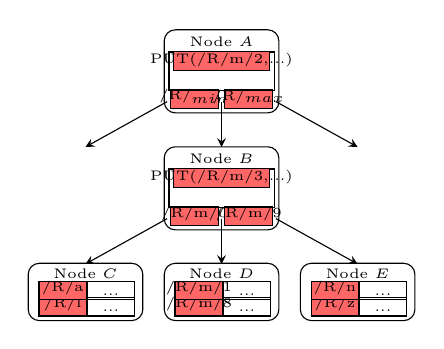
\begin{tikzpicture}[xscale=0.95, yscale=0.95]
            \node[anchor=south, rectangle, rounded corners, minimum height=.06\textwidth, minimum width=.12\textwidth, draw=black] at (0, 0) {};
            \node[anchor=south, font=\tiny] at (0, .036\textwidth) {Node $D$};
            \node[anchor=south, rectangle, minimum height=.015\textwidth, minimum width=.05\textwidth, draw=black, fill={red!60}] at (-.025\textwidth, .005\textwidth) {};
            \node[anchor=south, font=\tiny] at (-.025\textwidth, 0) {/R/m/8};
            \node[anchor=south, rectangle, minimum height=.015\textwidth, minimum width=.05\textwidth, draw=black] at (.028\textwidth, .005\textwidth) {};
            \node[anchor=south, font=\tiny] at (.028\textwidth, 0) {...};
            \node[anchor=south, rectangle, minimum height=.015\textwidth, minimum width=.05\textwidth, draw=black, fill={red!60}] at (-.025\textwidth, .023\textwidth) {};
            \node[anchor=south, font=\tiny] at (-.025\textwidth, .018\textwidth) {/R/m/1};
            \node[anchor=south, rectangle, minimum height=.015\textwidth, minimum width=.05\textwidth, draw=black] at (.028\textwidth, .023\textwidth) {};
            \node[anchor=south, font=\tiny] at (.028\textwidth, .018\textwidth) {...};

            \node[anchor=south, rectangle, rounded corners, minimum height=.06\textwidth, minimum width=.12\textwidth, draw=black] at (.15\textwidth, 0) {};
            \node[anchor=south, font=\tiny] at (.15\textwidth, .036\textwidth) {Node $E$};
            \node[anchor=south, rectangle, minimum height=.015\textwidth, minimum width=.05\textwidth, draw=black, fill={red!60}] at (.125\textwidth, .005\textwidth) {};
            \node[anchor=south, font=\tiny] at (.125\textwidth, 0) {/R/z};
            \node[anchor=south, rectangle, minimum height=.015\textwidth, minimum width=.05\textwidth, draw=black] at (.178\textwidth, .005\textwidth) {};
            \node[anchor=south, font=\tiny] at (.178\textwidth, 0) {...};
            \node[anchor=south, rectangle, minimum height=.015\textwidth, minimum width=.05\textwidth, draw=black, fill={red!60}] at (.125\textwidth, .023\textwidth) {};
            \node[anchor=south, font=\tiny] at (.125\textwidth, .018\textwidth) {/R/n};
            \node[anchor=south, rectangle, minimum height=.015\textwidth, minimum width=.05\textwidth, draw=black] at (.178\textwidth, .023\textwidth) {};
            \node[anchor=south, font=\tiny] at (.178\textwidth, .018\textwidth) {...};

            \node[anchor=south, rectangle, rounded corners, minimum height=.06\textwidth, minimum width=.12\textwidth, draw=black] at (-.15\textwidth, 0) {};
            \node[anchor=south, font=\tiny] at (-.15\textwidth, .036\textwidth) {Node $C$};
            \node[anchor=south, rectangle, minimum height=.015\textwidth, minimum width=.05\textwidth, draw=black, fill={red!60}] at (-.175\textwidth, .005\textwidth) {};
            \node[anchor=south, font=\tiny] at (-.175\textwidth, 0) {/R/l};
            \node[anchor=south, rectangle, minimum height=.015\textwidth, minimum width=.05\textwidth, draw=black] at (-.122\textwidth, .005\textwidth) {};
            \node[anchor=south, font=\tiny] at (-.122\textwidth, 0) {...};
            \node[anchor=south, rectangle, minimum height=.015\textwidth, minimum width=.05\textwidth, draw=black, fill={red!60}] at (-.175\textwidth, .023\textwidth) {};
            \node[anchor=south, font=\tiny] at (-.175\textwidth, .018\textwidth) {/R/a};
            \node[anchor=south, rectangle, minimum height=.015\textwidth, minimum width=.05\textwidth, draw=black] at (-.122\textwidth, .023\textwidth) {};
            \node[anchor=south, font=\tiny] at (-.122\textwidth, .018\textwidth) {...};

            \node[anchor=south, rectangle, rounded corners, minimum height=.087\textwidth, minimum width=.12\textwidth, draw=black, ] at (0, .1\textwidth) {};
            \node[anchor=south, font=\tiny] at (0, .163\textwidth) {Node $B$};
            \node[anchor=south, rectangle, minimum height=.015\textwidth, minimum width=.05\textwidth, draw=black, fill={red!60}] at (-.03\textwidth, .105\textwidth) {};
            \node[anchor=south, font=\tiny] at (-.03\textwidth, .1\textwidth) {/R/m/0};
            \node[anchor=south, rectangle, minimum height=.015\textwidth, minimum width=.05\textwidth, draw=black, fill={red!60}] at (.03\textwidth, .105\textwidth) {};
            \node[anchor=south, font=\tiny] at (.03\textwidth, .1\textwidth) {/R/m/9};
            \node[anchor=south, rectangle, minimum height=.04\textwidth, minimum width=.11\textwidth, draw=black] at (0, .125\textwidth) {};
            \node[anchor=south, rectangle, minimum height=.015\textwidth, minimum width=.1\textwidth, draw=black, fill={red!60}] at (0, .147\textwidth) {};
            \node[anchor=south, font=\tiny] at  (0, .141\textwidth) {PUT(/R/m/3,...)};

            \node[anchor=south, rectangle, rounded corners, minimum height=.087\textwidth, minimum width=.12\textwidth, draw=black] at (0, .229\textwidth) {};
            \node[anchor=south, font=\tiny] at (0, .292\textwidth) {Node $A$};
            \node[anchor=south, rectangle, minimum height=.015\textwidth, minimum width=.05\textwidth, draw=black, fill={red!60}] at (-.03\textwidth, .234\textwidth) {};
            \node[anchor=south, font=\tiny] at (-.03\textwidth, .229\textwidth) {/R/$_{min}$};
            \node[anchor=south, rectangle, minimum height=.015\textwidth, minimum width=.05\textwidth, draw=black, fill={red!60}] at (.03\textwidth, .234\textwidth) {};
            \node[anchor=south, font=\tiny] at (.03\textwidth, .229\textwidth) {/R/$_{max}$};
            \node[anchor=south, rectangle, minimum height=.04\textwidth, minimum width=.11\textwidth, draw=black] at (0, .254\textwidth) {};
            \node[anchor=south, rectangle, minimum height=.015\textwidth, minimum width=.1\textwidth, draw=black, fill={red!60}] at (0, .276\textwidth) {};
            \node[anchor=south, font=\tiny] at  (0, .27\textwidth) {PUT(/R/m/2,...)};

            \draw[->, >=stealth] (0, .113\textwidth) -- (0, .063\textwidth);
            \draw[->, >=stealth] (.06\textwidth, .113\textwidth) -- (.15\textwidth, .063\textwidth);
            \draw[->, >=stealth] (-.06\textwidth, .113\textwidth) -- (-.15\textwidth, .063\textwidth);
            \draw[->, >=stealth] (0, .242\textwidth) -- (0, .192\textwidth);
            \draw[->, >=stealth] (.06\textwidth, .242\textwidth) -- (.15\textwidth, .192\textwidth);
            \draw[->, >=stealth] (-.06\textwidth, .242\textwidth) -- (-.15\textwidth, .192\textwidth);
        \end{tikzpicture}
        \caption{\label{subfig:lift-0} A \bet without key lifting.}
    \end{subfigure}
    \begin{subfigure}{\textwidth}
        \centering
        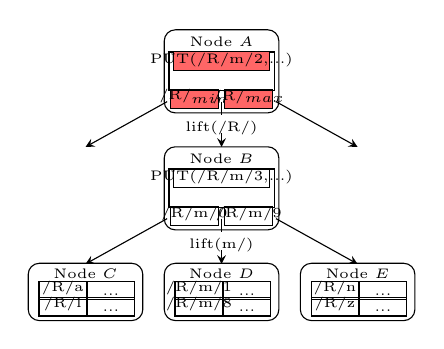
\begin{tikzpicture}[xscale=0.95, yscale=0.95]
            \node[anchor=south, rectangle, rounded corners, minimum height=.06\textwidth, minimum width=.12\textwidth, draw=black] at (0, 0) {};
            \node[anchor=south, font=\tiny] at (0, .036\textwidth) {Node $D$};
            \node[anchor=south, rectangle, minimum height=.015\textwidth, minimum width=.05\textwidth, draw=black] at (-.025\textwidth, .005\textwidth) {};
            \node[anchor=south, font=\tiny] at (-.025\textwidth, 0) {\st{/R/m/}8};
            \node[anchor=south, rectangle, minimum height=.015\textwidth, minimum width=.05\textwidth, draw=black] at (.028\textwidth, .005\textwidth) {};
            \node[anchor=south, font=\tiny] at (.028\textwidth, 0) {...};
            \node[anchor=south, rectangle, minimum height=.015\textwidth, minimum width=.05\textwidth, draw=black] at (-.025\textwidth, .023\textwidth) {};
            \node[anchor=south, font=\tiny] at (-.025\textwidth, .018\textwidth) {\st{/R/m/}1};
            \node[anchor=south, rectangle, minimum height=.015\textwidth, minimum width=.05\textwidth, draw=black] at (.028\textwidth, .023\textwidth) {};
            \node[anchor=south, font=\tiny] at (.028\textwidth, .018\textwidth) {...};

            \node[anchor=south, rectangle, rounded corners, minimum height=.06\textwidth, minimum width=.12\textwidth, draw=black] at (.15\textwidth, 0) {};
            \node[anchor=south, font=\tiny] at (.15\textwidth, .036\textwidth) {Node $E$};
            \node[anchor=south, rectangle, minimum height=.015\textwidth, minimum width=.05\textwidth, draw=black] at (.125\textwidth, .005\textwidth) {};
            \node[anchor=south, font=\tiny] at (.125\textwidth, 0) {\st{/R/}z};
            \node[anchor=south, rectangle, minimum height=.015\textwidth, minimum width=.05\textwidth, draw=black] at (.178\textwidth, .005\textwidth) {};
            \node[anchor=south, font=\tiny] at (.178\textwidth, 0) {...};
            \node[anchor=south, rectangle, minimum height=.015\textwidth, minimum width=.05\textwidth, draw=black] at (.125\textwidth, .023\textwidth) {};
            \node[anchor=south, font=\tiny] at (.125\textwidth, .018\textwidth) {\st{/R/}n};
            \node[anchor=south, rectangle, minimum height=.015\textwidth, minimum width=.05\textwidth, draw=black] at (.178\textwidth, .023\textwidth) {};
            \node[anchor=south, font=\tiny] at (.178\textwidth, .018\textwidth) {...};

            \node[anchor=south, rectangle, rounded corners, minimum height=.06\textwidth, minimum width=.12\textwidth, draw=black] at (-.15\textwidth, 0) {};
            \node[anchor=south, font=\tiny] at (-.15\textwidth, .036\textwidth) {Node $C$};
            \node[anchor=south, rectangle, minimum height=.015\textwidth, minimum width=.05\textwidth, draw=black] at (-.175\textwidth, .005\textwidth) {};
            \node[anchor=south, font=\tiny] at (-.175\textwidth, 0) {\st{/R/}l};
            \node[anchor=south, rectangle, minimum height=.015\textwidth, minimum width=.05\textwidth, draw=black] at (-.122\textwidth, .005\textwidth) {};
            \node[anchor=south, font=\tiny] at (-.122\textwidth, 0) {...};
            \node[anchor=south, rectangle, minimum height=.015\textwidth, minimum width=.05\textwidth, draw=black] at (-.175\textwidth, .023\textwidth) {};
            \node[anchor=south, font=\tiny] at (-.175\textwidth, .018\textwidth) {\st{/R/}a};
            \node[anchor=south, rectangle, minimum height=.015\textwidth, minimum width=.05\textwidth, draw=black] at (-.122\textwidth, .023\textwidth) {};
            \node[anchor=south, font=\tiny] at (-.122\textwidth, .018\textwidth) {...};

            \node[anchor=south, rectangle, rounded corners, minimum height=.087\textwidth, minimum width=.12\textwidth, draw=black] at (0, .1\textwidth) {};
            \node[anchor=south, font=\tiny] at (0, .163\textwidth) {Node $B$};
            \node[anchor=south, rectangle, minimum height=.015\textwidth, minimum width=.05\textwidth, draw=black] at (-.03\textwidth, .105\textwidth) {};
            \node[anchor=south, font=\tiny] at (-.03\textwidth, .1\textwidth) {\st{/R/}m/0};
            \node[anchor=south, rectangle, minimum height=.015\textwidth, minimum width=.05\textwidth, draw=black] at (.03\textwidth, .105\textwidth) {};
            \node[anchor=south, font=\tiny] at (.03\textwidth, .1\textwidth) {\st{/R/}m/9};
            \node[anchor=south, rectangle, minimum height=.04\textwidth, minimum width=.11\textwidth, draw=black] at (0, .125\textwidth) {};
            \node[anchor=south, rectangle, minimum height=.015\textwidth, minimum width=.1\textwidth, draw=black] at (0, .147\textwidth) {};
            \node[anchor=south, font=\tiny] at  (0, .141\textwidth) {PUT(\st{/R/}m/3,...)};

            \node[anchor=south, rectangle, rounded corners, minimum height=.087\textwidth, minimum width=.12\textwidth, draw=black] at (0, .229\textwidth) {};
            \node[anchor=south, font=\tiny] at (0, .292\textwidth) {Node $A$};
            \node[anchor=south, rectangle, minimum height=.015\textwidth, minimum width=.05\textwidth, draw=black, fill={red!60}] at (-.03\textwidth, .234\textwidth) {};
            \node[anchor=south, font=\tiny] at (-.03\textwidth, .229\textwidth) {/R/$_{min}$};
            \node[anchor=south, rectangle, minimum height=.015\textwidth, minimum width=.05\textwidth, draw=black, fill={red!60}] at (.03\textwidth, .234\textwidth) {};
            \node[anchor=south, font=\tiny] at (.03\textwidth, .229\textwidth) {/R/$_{max}$};
            \node[anchor=south, rectangle, minimum height=.04\textwidth, minimum width=.11\textwidth, draw=black] at (0, .254\textwidth) {};
            \node[anchor=south, rectangle, minimum height=.015\textwidth, minimum width=.1\textwidth, draw=black, fill={red!60}] at (0, .276\textwidth) {};
            \node[anchor=south, font=\tiny] at  (0, .27\textwidth) {PUT(/R/m/2,...)};

            \draw[->, >=stealth] (0, .113\textwidth) -- (0, .063\textwidth);
            \draw[->, >=stealth] (.06\textwidth, .113\textwidth) -- (.15\textwidth, .063\textwidth);
            \draw[->, >=stealth] (-.06\textwidth, .113\textwidth) -- (-.15\textwidth, .063\textwidth);
            \draw[->, >=stealth] (0, .242\textwidth) -- (0, .192\textwidth);
            \draw[->, >=stealth] (.06\textwidth, .242\textwidth) -- (.15\textwidth, .192\textwidth);
            \draw[->, >=stealth] (-.06\textwidth, .242\textwidth) -- (-.15\textwidth, .192\textwidth);

            \node[anchor=north,rectangle, minimum height=.015\textwidth, minimum width=.05\textwidth, fill={white}] at (0, .228\textwidth) {};
            \node[anchor=north, font=\tiny] at (0, .231\textwidth) {lift(/R/)};
            \node[anchor=north,rectangle, minimum height=.015\textwidth, minimum width=.05\textwidth, fill={white}] at (0, .099\textwidth) {};
            \node[anchor=north, font=\tiny] at (0, .102\textwidth) {lift(m/)};
        \end{tikzpicture}
        \caption{\label{subfig:lift-1} The same tree with key lifting. Lifted prefixes are marked as strike-through in keys.}
    \end{subfigure}
    \begin{subfigure}{\textwidth}
        \centering
        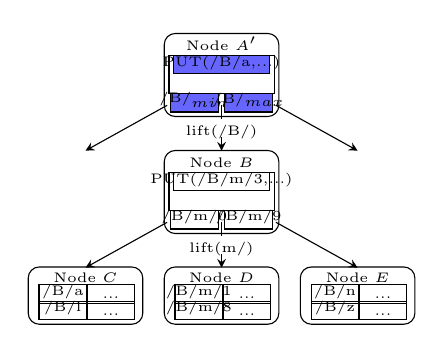
\begin{tikzpicture}[xscale=0.95, yscale=0.95]
            \node[anchor=south, rectangle, rounded corners, minimum height=.06\textwidth, minimum width=.12\textwidth, draw=black] at (0, 0) {};
            \node[anchor=south, font=\tiny] at (0, .036\textwidth) {Node $D$};
            \node[anchor=south, rectangle, minimum height=.015\textwidth, minimum width=.05\textwidth, draw=black] at (-.025\textwidth, .005\textwidth) {};
            \node[anchor=south, font=\tiny] at (-.025\textwidth, 0) {\st{/B/m/}8};
            \node[anchor=south, rectangle, minimum height=.015\textwidth, minimum width=.05\textwidth, draw=black] at (.028\textwidth, .005\textwidth) {};
            \node[anchor=south, font=\tiny] at (.028\textwidth, 0) {...};
            \node[anchor=south, rectangle, minimum height=.015\textwidth, minimum width=.05\textwidth, draw=black] at (-.025\textwidth, .023\textwidth) {};
            \node[anchor=south, font=\tiny] at (-.025\textwidth, .018\textwidth) {\st{/B/m/}1};
            \node[anchor=south, rectangle, minimum height=.015\textwidth, minimum width=.05\textwidth, draw=black] at (.028\textwidth, .023\textwidth) {};
            \node[anchor=south, font=\tiny] at (.028\textwidth, .018\textwidth) {...};

            \node[anchor=south, rectangle, rounded corners, minimum height=.06\textwidth, minimum width=.12\textwidth, draw=black] at (.15\textwidth, 0) {};
            \node[anchor=south, font=\tiny] at (.15\textwidth, .036\textwidth) {Node $E$};
            \node[anchor=south, rectangle, minimum height=.015\textwidth, minimum width=.05\textwidth, draw=black] at (.125\textwidth, .005\textwidth) {};
            \node[anchor=south, font=\tiny] at (.125\textwidth, 0) {\st{/B/}z};
            \node[anchor=south, rectangle, minimum height=.015\textwidth, minimum width=.05\textwidth, draw=black] at (.178\textwidth, .005\textwidth) {};
            \node[anchor=south, font=\tiny] at (.178\textwidth, 0) {...};
            \node[anchor=south, rectangle, minimum height=.015\textwidth, minimum width=.05\textwidth, draw=black] at (.125\textwidth, .023\textwidth) {};
            \node[anchor=south, font=\tiny] at (.125\textwidth, .018\textwidth) {\st{/B/}n};
            \node[anchor=south, rectangle, minimum height=.015\textwidth, minimum width=.05\textwidth, draw=black] at (.178\textwidth, .023\textwidth) {};
            \node[anchor=south, font=\tiny] at (.178\textwidth, .018\textwidth) {...};

            \node[anchor=south, rectangle, rounded corners, minimum height=.06\textwidth, minimum width=.12\textwidth, draw=black] at (-.15\textwidth, 0) {};
            \node[anchor=south, font=\tiny] at (-.15\textwidth, .036\textwidth) {Node $C$};
            \node[anchor=south, rectangle, minimum height=.015\textwidth, minimum width=.05\textwidth, draw=black] at (-.175\textwidth, .005\textwidth) {};
            \node[anchor=south, font=\tiny] at (-.175\textwidth, 0) {\st{/B/}l};
            \node[anchor=south, rectangle, minimum height=.015\textwidth, minimum width=.05\textwidth, draw=black] at (-.122\textwidth, .005\textwidth) {};
            \node[anchor=south, font=\tiny] at (-.122\textwidth, 0) {...};
            \node[anchor=south, rectangle, minimum height=.015\textwidth, minimum width=.05\textwidth, draw=black] at (-.175\textwidth, .023\textwidth) {};
            \node[anchor=south, font=\tiny] at (-.175\textwidth, .018\textwidth) {\st{/B/}a};
            \node[anchor=south, rectangle, minimum height=.015\textwidth, minimum width=.05\textwidth, draw=black] at (-.122\textwidth, .023\textwidth) {};
            \node[anchor=south, font=\tiny] at (-.122\textwidth, .018\textwidth) {...};

            \node[anchor=south, rectangle, rounded corners, minimum height=.087\textwidth, minimum width=.12\textwidth, draw=black] at (0, .1\textwidth) {};
            \node[anchor=south, font=\tiny] at (0, .163\textwidth) {Node $B$};
            \node[anchor=south, rectangle, minimum height=.015\textwidth, minimum width=.05\textwidth, draw=black] at (-.03\textwidth, .105\textwidth) {};
            \node[anchor=south, font=\tiny] at (-.03\textwidth, .1\textwidth) {\st{/B/}m/0};
            \node[anchor=south, rectangle, minimum height=.015\textwidth, minimum width=.05\textwidth, draw=black] at (.03\textwidth, .105\textwidth) {};
            \node[anchor=south, font=\tiny] at (.03\textwidth, .1\textwidth) {\st{/B/}m/9};
            \node[anchor=south, rectangle, minimum height=.04\textwidth, minimum width=.11\textwidth, draw=black] at (0, .125\textwidth) {};
            \node[anchor=south, rectangle, minimum height=.015\textwidth, minimum width=.1\textwidth, draw=black] at (0, .147\textwidth) {};
            \node[anchor=south, font=\tiny] at  (0, .141\textwidth) {PUT(\st{/B/}m/3,...)};

            \node[anchor=south, rectangle, rounded corners, minimum height=.087\textwidth, minimum width=.12\textwidth, draw=black] at (0, .229\textwidth) {};
            \node[anchor=south, font=\tiny] at (0, .292\textwidth) {Node $A'$};
            \node[anchor=south, rectangle, minimum height=.015\textwidth, minimum width=.05\textwidth, draw=black, fill={blue!60}] at (-.03\textwidth, .234\textwidth) {};
            \node[anchor=south, font=\tiny] at (-.03\textwidth, .229\textwidth) {/B/$_{min}$};
            \node[anchor=south, rectangle, minimum height=.015\textwidth, minimum width=.05\textwidth, draw=black, fill={blue!60}] at (.03\textwidth, .234\textwidth) {};
            \node[anchor=south, font=\tiny] at (.03\textwidth, .229\textwidth) {/B/$_{max}$};
            \node[anchor=south, rectangle, minimum height=.04\textwidth, minimum width=.11\textwidth, draw=black] at (0, .254\textwidth) {};
            \node[anchor=south, rectangle, minimum height=.015\textwidth, minimum width=.1\textwidth, draw=black, fill={blue!60}] at (0, .276\textwidth) {};
            \node[anchor=south, font=\tiny] at  (0, .27\textwidth) {PUT(/B/a,...)};

            \draw[->, >=stealth] (0, .113\textwidth) -- (0, .063\textwidth);
            \draw[->, >=stealth] (.06\textwidth, .113\textwidth) -- (.15\textwidth, .063\textwidth);
            \draw[->, >=stealth] (-.06\textwidth, .113\textwidth) -- (-.15\textwidth, .063\textwidth);
            \draw[->, >=stealth] (0, .242\textwidth) -- (0, .192\textwidth);
            \draw[->, >=stealth] (.06\textwidth, .242\textwidth) -- (.15\textwidth, .192\textwidth);
            \draw[->, >=stealth] (-.06\textwidth, .242\textwidth) -- (-.15\textwidth, .192\textwidth);

            \node[anchor=north,rectangle, minimum height=.015\textwidth, minimum width=.05\textwidth, fill={white}] at (0, .228\textwidth) {};
            \node[anchor=north, font=\tiny] at (0, .231\textwidth) {lift(/B/)};
            \node[anchor=north,rectangle, minimum height=.015\textwidth, minimum width=.05\textwidth, fill={white}] at (0, .099\textwidth) {};
            \node[anchor=north, font=\tiny] at (0, .102\textwidth) {lift(m/)};
        \end{tikzpicture}
        \caption{\label{subfig:lift-2} When the subtree rooted at Node $B$ is bounded by different pivots, all keys in the subtree change their prefixes.}
    \end{subfigure}
    \caption[Key lifting example]{\label{fig:lift}
        Key lifting lifts prefixes from the subtree. Keys in the same subtree
        are viewed with different prefixes when the pivots in its parent
        changes.}
\end{figure}

After tree surgery, one can move the isolated subtree to another location on
the \bet.
However, the keys in the subtree will not be coherent with the new location in
the tree.
As part of a range-rename, the prefixes of keys in this subtree need to be
updated.
Updating the prefixes by traversing the subtree costs a lot of IOs, touching
nodes that would otherwise be untouched by the tree surgery.
The particularly concerning case is when the subtree is a very large.

Key lifting eliminates the need to update prefixes in the subtree by
transforming \bets to lifted \bets.
The idea of key lifting comes from the observation that with lexicographic key
order, all keys in the range of two pivots must have the same prefix that is
the \textbf{LCP} (Longest Common Prefix) of the pivots.
Therefore, this LCP is redundant information in the subtree of the two pivots
and can be removed from the subtree.
In particular, the subtree generated by tree surgery is bounded by two pivots,
$p_{min}$ and $p_{max}$ and with lexicographic key order, all keys in the
subtree must have prefix $p$.

In lifted \bets, a parent-to-child pointer lifts the LCP of the two pivots from
the subtree rooted at the child.
Child nodes only store differing key suffixes.
This approach encodes the complete key in the path taken to reach a given node
and one can then modify the prefix for a lifted subtree by only modifying the
parent node, eliminating the need to change key and pivot prefixes in all nodes
of a subtree.

For example, in Figure~\ref{subfig:lift-1}, the subtree rooted at Node $B$ is
bounded by ``/R/$_{min}$'' and ``/R/$_{max}$'' in Node $A$.
Therefore, all keys in the subtree must have prefix ``/R/'' and key lifting
removes this prefix from the subtree (marked as strike-through in keys).
Likewise, Node $D$ is bounded by ``m/a'' and ``m/z'' in Node $B$
(note ``/R/'' is already lifted from the sutbree rooted at Node $B$),
so key lifting removes the prefix ``m/'' from Node $D$.
In Figure~\ref{subfig:lift-2}, the same subtree, which contains exactly the
same key/value pairs, is moved to a different location, bounded by
``/B/$_{min}$'' and ``/B/$_{max}$'' in Node $A'$.
Because the prefix lifted through the parent-to-child pointer in Node $A'$
becomes ``/B/'', all keys in the subtree have ``/B/'' prefixes instead.

Key lifting doesn't introduce additional IOs to operations on \bets.
A query on a lifted \bet needs to memorize lifted prefixes during the
root-to-leaf traversal and reconstruct the full key by concatenating these
prefixes and the suffix in the leaf.
Lifted \bets must remove the lifted prefix from a message before flushing the
message from parent to child.
A node split in a lifted \bet adds a pivot to the parent, changing the lifted
prefix in the parent-to-child pointer, so it needs to update keys in the
resulting children.
However, this doesn't incur additional IO.
Similarly, no additional IO is required in node merges.

Key lifting is completely transparent to the application using the key/value
store.
From \betrfs's perspective, it is still storing key/value pairs with
full-path keys, just with a slightly different data structure.

\subsection{Range-rename on lifted \bets}

\begin{figure}
    \begin{subfigure}{\textwidth}
        \centering
        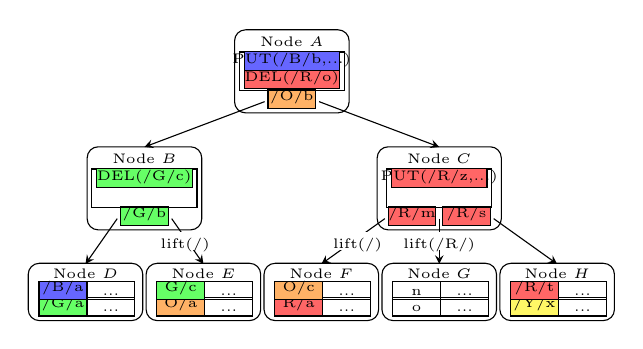
\begin{tikzpicture}[xscale=0.95, yscale=0.95]
            \node[anchor=south, rectangle, rounded corners, minimum height=.06\textwidth, minimum width=.12\textwidth, draw=black] at (0, 0) {};
            \node[anchor=south, font=\tiny] at (0, .036\textwidth) {Node $F$};
            \node[anchor=south, rectangle, minimum height=.015\textwidth, minimum width=.05\textwidth, draw=black, fill={red!60}] at (-.025\textwidth, .005\textwidth) {};
            \node[anchor=south, font=\tiny] at (-.025\textwidth, 0) {R/a};
            \node[anchor=south, rectangle, minimum height=.015\textwidth, minimum width=.05\textwidth, draw=black] at (.028\textwidth, .005\textwidth) {};
            \node[anchor=south, font=\tiny] at (.028\textwidth, 0) {...};
            \node[anchor=south, rectangle, minimum height=.015\textwidth, minimum width=.05\textwidth, draw=black, fill={orange!60}] at (-.025\textwidth, .023\textwidth) {};
            \node[anchor=south, font=\tiny] at (-.025\textwidth, .018\textwidth) {O/c};
            \node[anchor=south, rectangle, minimum height=.015\textwidth, minimum width=.05\textwidth, draw=black] at (.028\textwidth, .023\textwidth) {};
            \node[anchor=south, font=\tiny] at (.028\textwidth, .018\textwidth) {...};

            \node[anchor=south, rectangle, rounded corners, minimum height=.06\textwidth, minimum width=.12\textwidth, draw=black] at (.13\textwidth, 0) {};
            \node[anchor=south, font=\tiny] at (.13\textwidth, .036\textwidth) {Node $G$};
            \node[anchor=south, rectangle, minimum height=.015\textwidth, minimum width=.05\textwidth, draw=black] at (.105\textwidth, .005\textwidth) {};
            \node[anchor=south, font=\tiny] at (.105\textwidth, 0) {o};
            \node[anchor=south, rectangle, minimum height=.015\textwidth, minimum width=.05\textwidth, draw=black] at (.158\textwidth, .005\textwidth) {};
            \node[anchor=south, font=\tiny] at (.158\textwidth, 0) {...};
            \node[anchor=south, rectangle, minimum height=.015\textwidth, minimum width=.05\textwidth, draw=black] at (.105\textwidth, .023\textwidth) {};
            \node[anchor=south, font=\tiny] at (.105\textwidth, .018\textwidth) {n};
            \node[anchor=south, rectangle, minimum height=.015\textwidth, minimum width=.05\textwidth, draw=black] at (.158\textwidth, .023\textwidth) {};
            \node[anchor=south, font=\tiny] at (.158\textwidth, .018\textwidth) {...};

            \node[anchor=south, rectangle, rounded corners, minimum height=.06\textwidth, minimum width=.12\textwidth, draw=black] at (.26\textwidth, 0) {};
            \node[anchor=south, font=\tiny] at (.26\textwidth, .036\textwidth) {Node $H$};
            \node[anchor=south, rectangle, minimum height=.015\textwidth, minimum width=.05\textwidth, draw=black, fill={yellow!60}] at (.235\textwidth, .005\textwidth) {};
            \node[anchor=south, font=\tiny] at (.235\textwidth, 0) {/Y/x};
            \node[anchor=south, rectangle, minimum height=.015\textwidth, minimum width=.05\textwidth, draw=black] at (.288\textwidth, .005\textwidth) {};
            \node[anchor=south, font=\tiny] at (.288\textwidth, 0) {...};
            \node[anchor=south, rectangle, minimum height=.015\textwidth, minimum width=.05\textwidth, draw=black, fill={red!60}] at (.235\textwidth, .023\textwidth) {};
            \node[anchor=south, font=\tiny] at (.235\textwidth, .018\textwidth) {/R/t};
            \node[anchor=south, rectangle, minimum height=.015\textwidth, minimum width=.05\textwidth, draw=black] at (.288\textwidth, .023\textwidth) {};
            \node[anchor=south, font=\tiny] at (.288\textwidth, .018\textwidth) {...};

            \node[anchor=south, rectangle, rounded corners, minimum height=.06\textwidth, minimum width=.12\textwidth, draw=black] at (-.13\textwidth, 0) {};
            \node[anchor=south, font=\tiny] at (-.13\textwidth, .036\textwidth) {Node $E$};
            \node[anchor=south, rectangle, minimum height=.015\textwidth, minimum width=.05\textwidth, draw=black, fill={orange!60}] at (-.155\textwidth, .005\textwidth) {};
            \node[anchor=south, font=\tiny] at (-.155\textwidth, 0) {O/a};
            \node[anchor=south, rectangle, minimum height=.015\textwidth, minimum width=.05\textwidth, draw=black] at (-.102\textwidth, .005\textwidth) {};
            \node[anchor=south, font=\tiny] at (-.102\textwidth, 0) {...};
            \node[anchor=south, rectangle, minimum height=.015\textwidth, minimum width=.05\textwidth, draw=black, fill={green!60}] at (-.155\textwidth, .023\textwidth) {};
            \node[anchor=south, font=\tiny] at (-.155\textwidth, .018\textwidth) {G/c};
            \node[anchor=south, rectangle, minimum height=.015\textwidth, minimum width=.05\textwidth, draw=black] at (-.102\textwidth, .023\textwidth) {};
            \node[anchor=south, font=\tiny] at (-.102\textwidth, .018\textwidth) {...};

            \node[anchor=south, rectangle, rounded corners, minimum height=.06\textwidth, minimum width=.12\textwidth, draw=black] at (-.26\textwidth, 0) {};
            \node[anchor=south, font=\tiny] at (-.26\textwidth, .036\textwidth) {Node $D$};
            \node[anchor=south, rectangle, minimum height=.015\textwidth, minimum width=.05\textwidth, draw=black, fill={green!60}] at (-.285\textwidth, .005\textwidth) {};
            \node[anchor=south, font=\tiny] at (-.285\textwidth, 0) {/G/a};
            \node[anchor=south, rectangle, minimum height=.015\textwidth, minimum width=.05\textwidth, draw=black] at (-.232\textwidth, .005\textwidth) {};
            \node[anchor=south, font=\tiny] at (-.232\textwidth, 0) {...};
            \node[anchor=south, rectangle, minimum height=.015\textwidth, minimum width=.05\textwidth, draw=black, fill={blue!60}] at (-.285\textwidth, .023\textwidth) {};
            \node[anchor=south, font=\tiny] at (-.285\textwidth, .018\textwidth) {/B/a};
            \node[anchor=south, rectangle, minimum height=.015\textwidth, minimum width=.05\textwidth, draw=black] at (-.232\textwidth, .023\textwidth) {};
            \node[anchor=south, font=\tiny] at (-.232\textwidth, .018\textwidth) {...};

            \node[anchor=south, rectangle, rounded corners, minimum height=.087\textwidth, minimum width=.12\textwidth, draw=black] at (-.195\textwidth, .1\textwidth) {};
            \node[anchor=south, font=\tiny] at (-.195\textwidth, .163\textwidth) {Node $B$};
            \node[anchor=south, rectangle, minimum height=.015\textwidth, minimum width=.05\textwidth, draw=black, fill={green!60}] at (-.195\textwidth, .105\textwidth) {};
            \node[anchor=south, font=\tiny] at (-.195\textwidth, .1\textwidth) {/G/b};
            \node[anchor=south, rectangle, minimum height=.04\textwidth, minimum width=.11\textwidth, draw=black] at (-.195\textwidth, .125\textwidth) {};
            \node[anchor=south, rectangle, minimum height=.015\textwidth, minimum width=.1\textwidth, draw=black, fill={green!60}] at (-.195\textwidth, .147\textwidth) {};
            \node[anchor=south, font=\tiny] at  (-.195\textwidth, .141\textwidth) {DEL(/G/c)};

            \node[anchor=south, rectangle, rounded corners, minimum height=.087\textwidth, minimum width=.13\textwidth, draw=black] at (.13\textwidth, .1\textwidth) {};
            \node[anchor=south, font=\tiny] at (.13\textwidth, .163\textwidth) {Node $C$};
            \node[anchor=south, rectangle, minimum height=.015\textwidth, minimum width=.05\textwidth, draw=black, fill={red!60}] at (.1\textwidth, .105\textwidth) {};
            \node[anchor=south, font=\tiny] at (.1\textwidth, .1\textwidth) {/R/m};
            \node[anchor=south, rectangle, minimum height=.015\textwidth, minimum width=.05\textwidth, draw=black, fill={red!60}] at (.16\textwidth, .105\textwidth) {};
            \node[anchor=south, font=\tiny] at (.16\textwidth, .1\textwidth) {/R/s};
            \node[anchor=south, rectangle, minimum height=.04\textwidth, minimum width=.11\textwidth, draw=black] at (.13\textwidth, .125\textwidth) {};
            \node[anchor=south, rectangle, minimum height=.015\textwidth, minimum width=.1\textwidth, draw=black, fill={red!60}] at (.13\textwidth, .147\textwidth) {};
            \node[anchor=south, font=\tiny] at  (.13\textwidth, .141\textwidth) {PUT(/R/z,...)};

            \node[anchor=south, rectangle, rounded corners, minimum height=.087\textwidth, minimum width=.12\textwidth, draw=black] at (-.0325\textwidth, .229\textwidth) {};
            \node[anchor=south, font=\tiny] at (-.0325\textwidth, .292\textwidth) {Node $A$};
            \node[anchor=south, rectangle, minimum height=.015\textwidth, minimum width=.05\textwidth, draw=black, fill={orange!60}] at (-.0325\textwidth, .234\textwidth) {};
            \node[anchor=south, font=\tiny] at (-.0325\textwidth, .229\textwidth) {/O/b};
            \node[anchor=south, rectangle, minimum height=.04\textwidth, minimum width=.11\textwidth, draw=black] at (-.0325\textwidth, .254\textwidth) {};
            \node[anchor=south, rectangle, minimum height=.015\textwidth, minimum width=.1\textwidth, draw=black, fill={red!60}] at (-.0325\textwidth, .256\textwidth) {};
            \node[anchor=south, font=\tiny] at  (-.0325\textwidth, .25\textwidth) {DEL(/R/o)};
            \node[anchor=south, rectangle, minimum height=.015\textwidth, minimum width=.1\textwidth, draw=black, fill={blue!60}] at (-.0325\textwidth, .276\textwidth) {};
            \node[anchor=south, font=\tiny] at  (-.0325\textwidth, .27\textwidth) {PUT(/B/b,...)};

            \draw[->, >=stealth] (-.225\textwidth, .113\textwidth) -- (-.26\textwidth, .063\textwidth);
            \draw[->, >=stealth] (-.165\textwidth, .113\textwidth) -- (-.13\textwidth, .063\textwidth);
            \draw[->, >=stealth] (.13\textwidth, .113\textwidth) -- (.13\textwidth, .063\textwidth);
            \draw[->, >=stealth] (.19\textwidth, .113\textwidth) -- (.26\textwidth, .063\textwidth);
            \draw[->, >=stealth] (.07\textwidth, .113\textwidth) -- (0, .063\textwidth);
            \draw[->, >=stealth] (-.0625\textwidth, .242\textwidth) -- (-.195\textwidth, .192\textwidth);
            \draw[->, >=stealth] (-.0025\textwidth, .242\textwidth) -- (.13\textwidth, .192\textwidth);

            \node[anchor=north,rectangle, minimum height=.015\textwidth, minimum width=.05\textwidth, fill={white}] at (.13\textwidth, .099\textwidth) {};
            \node[anchor=north, font=\tiny] at (.13\textwidth, .102\textwidth) {lift(/R/)};
            \node[anchor=north,rectangle, minimum height=.015\textwidth, minimum width=.05\textwidth, fill={white}] at (.04\textwidth, .099\textwidth) {};
            \node[anchor=north, font=\tiny] at (.04\textwidth, .102\textwidth) {lift(/)};
            \node[anchor=north,rectangle, minimum height=.015\textwidth, minimum width=.05\textwidth, fill={white}] at (-.15\textwidth, .099\textwidth) {};
            \node[anchor=north, font=\tiny] at (-.15\textwidth, .102\textwidth) {lift(/)};
        \end{tikzpicture}
        \caption{\label{subfig:rr-1} The \bet before the range-rename.}
    \end{subfigure}
    \begin{subfigure}{\textwidth}
        \centering
        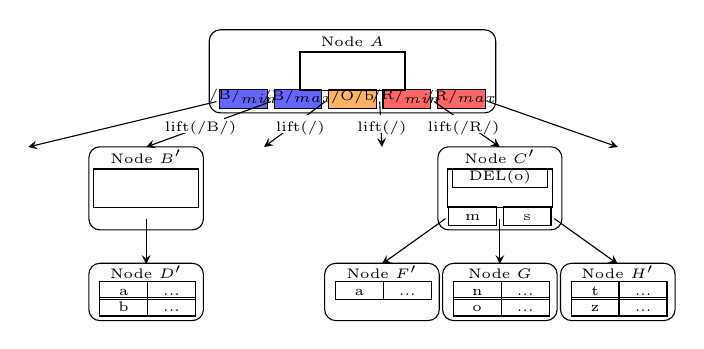
\begin{tikzpicture}[xscale=0.95, yscale=0.95]
            \node[anchor=south, rectangle, rounded corners, minimum height=.06\textwidth, minimum width=.12\textwidth, draw=black] at (0, 0) {};
            \node[anchor=south, font=\tiny] at (0, .036\textwidth) {Node $F'$};
            \node[anchor=south, rectangle, minimum height=.015\textwidth, minimum width=.05\textwidth, draw=black] at (-.025\textwidth, .023\textwidth) {};
            \node[anchor=south, font=\tiny] at (-.025\textwidth, .018\textwidth) {a};
            \node[anchor=south, rectangle, minimum height=.015\textwidth, minimum width=.05\textwidth, draw=black] at (.028\textwidth, .023\textwidth) {};
            \node[anchor=south, font=\tiny] at (.028\textwidth, .018\textwidth) {...};

            \node[anchor=south, rectangle, rounded corners, minimum height=.06\textwidth, minimum width=.12\textwidth, draw=black] at (.13\textwidth, 0) {};
            \node[anchor=south, font=\tiny] at (.13\textwidth, .036\textwidth) {Node $G$};
            \node[anchor=south, rectangle, minimum height=.015\textwidth, minimum width=.05\textwidth, draw=black] at (.105\textwidth, .005\textwidth) {};
            \node[anchor=south, font=\tiny] at (.105\textwidth, 0) {o};
            \node[anchor=south, rectangle, minimum height=.015\textwidth, minimum width=.05\textwidth, draw=black] at (.158\textwidth, .005\textwidth) {};
            \node[anchor=south, font=\tiny] at (.158\textwidth, 0) {...};
            \node[anchor=south, rectangle, minimum height=.015\textwidth, minimum width=.05\textwidth, draw=black] at (.105\textwidth, .023\textwidth) {};
            \node[anchor=south, font=\tiny] at (.105\textwidth, .018\textwidth) {n};
            \node[anchor=south, rectangle, minimum height=.015\textwidth, minimum width=.05\textwidth, draw=black] at (.158\textwidth, .023\textwidth) {};
            \node[anchor=south, font=\tiny] at (.158\textwidth, .018\textwidth) {...};

            \node[anchor=south, rectangle, rounded corners, minimum height=.06\textwidth, minimum width=.12\textwidth, draw=black] at (.26\textwidth, 0) {};
            \node[anchor=south, font=\tiny] at (.26\textwidth, .036\textwidth) {Node $H'$};
            \node[anchor=south, rectangle, minimum height=.015\textwidth, minimum width=.05\textwidth, draw=black] at (.235\textwidth, .005\textwidth) {};
            \node[anchor=south, font=\tiny] at (.235\textwidth, 0) {z};
            \node[anchor=south, rectangle, minimum height=.015\textwidth, minimum width=.05\textwidth, draw=black] at (.288\textwidth, .005\textwidth) {};
            \node[anchor=south, font=\tiny] at (.288\textwidth, 0) {...};
            \node[anchor=south, rectangle, minimum height=.015\textwidth, minimum width=.05\textwidth, draw=black] at (.235\textwidth, .023\textwidth) {};
            \node[anchor=south, font=\tiny] at (.235\textwidth, .018\textwidth) {t};
            \node[anchor=south, rectangle, minimum height=.015\textwidth, minimum width=.05\textwidth, draw=black] at (.288\textwidth, .023\textwidth) {};
            \node[anchor=south, font=\tiny] at (.288\textwidth, .018\textwidth) {...};

            \node[anchor=south, rectangle, rounded corners, minimum height=.06\textwidth, minimum width=.12\textwidth, draw=black] at (-.26\textwidth, 0) {};
            \node[anchor=south, font=\tiny] at (-.26\textwidth, .036\textwidth) {Node $D'$};
            \node[anchor=south, rectangle, minimum height=.015\textwidth, minimum width=.05\textwidth, draw=black] at (-.285\textwidth, .005\textwidth) {};
            \node[anchor=south, font=\tiny] at (-.285\textwidth, 0) {b};
            \node[anchor=south, rectangle, minimum height=.015\textwidth, minimum width=.05\textwidth, draw=black] at (-.232\textwidth, .005\textwidth) {};
            \node[anchor=south, font=\tiny] at (-.232\textwidth, 0) {...};
            \node[anchor=south, rectangle, minimum height=.015\textwidth, minimum width=.05\textwidth, draw=black] at (-.285\textwidth, .023\textwidth) {};
            \node[anchor=south, font=\tiny] at (-.285\textwidth, .018\textwidth) {a};
            \node[anchor=south, rectangle, minimum height=.015\textwidth, minimum width=.05\textwidth, draw=black] at (-.232\textwidth, .023\textwidth) {};
            \node[anchor=south, font=\tiny] at (-.232\textwidth, .018\textwidth) {...};

            \node[anchor=south, rectangle, rounded corners, minimum height=.087\textwidth, minimum width=.12\textwidth, draw=black] at (-.26\textwidth, .1\textwidth) {};
            \node[anchor=south, font=\tiny] at (-.26\textwidth, .163\textwidth) {Node $B'$};
            \node[anchor=south, rectangle, minimum height=.04\textwidth, minimum width=.11\textwidth, draw=black] at (-.26\textwidth, .125\textwidth) {};

            \node[anchor=south, rectangle, rounded corners, minimum height=.087\textwidth, minimum width=.13\textwidth, draw=black] at (.13\textwidth, .1\textwidth) {};
            \node[anchor=south, font=\tiny] at (.13\textwidth, .163\textwidth) {Node $C'$};
            \node[anchor=south, rectangle, minimum height=.015\textwidth, minimum width=.05\textwidth, draw=black] at (.1\textwidth, .105\textwidth) {};
            \node[anchor=south, font=\tiny] at (.1\textwidth, .1\textwidth) {m};
            \node[anchor=south, rectangle, minimum height=.015\textwidth, minimum width=.05\textwidth, draw=black] at (.16\textwidth, .105\textwidth) {};
            \node[anchor=south, font=\tiny] at (.16\textwidth, .1\textwidth) {s};
            \node[anchor=south, rectangle, minimum height=.04\textwidth, minimum width=.11\textwidth, draw=black] at (.13\textwidth, .125\textwidth) {};
            \node[anchor=south, rectangle, minimum height=.015\textwidth, minimum width=.1\textwidth, draw=black] at (.13\textwidth, .147\textwidth) {};
            \node[anchor=south, font=\tiny] at  (.13\textwidth, .141\textwidth) {DEL(o)};

            \node[anchor=south, rectangle, rounded corners, minimum height=.087\textwidth, minimum width=.3\textwidth, draw=black] at (-.0325\textwidth, .229\textwidth) {};
            \node[anchor=south, font=\tiny] at (-.0325\textwidth, .292\textwidth) {Node $A$};
            \node[anchor=south, rectangle, minimum height=.015\textwidth, minimum width=.05\textwidth, draw=black, fill={blue!60}] at (-.1525\textwidth, .234\textwidth) {};
            \node[anchor=south, font=\tiny] at (-.1525\textwidth, .229\textwidth) {/B/$_{min}$};
            \node[anchor=south, rectangle, minimum height=.015\textwidth, minimum width=.05\textwidth, draw=black, fill={blue!60}] at (-.0925\textwidth, .234\textwidth) {};
            \node[anchor=south, font=\tiny] at (-.0925\textwidth, .229\textwidth) {/B/$_{max}$};
            \node[anchor=south, rectangle, minimum height=.015\textwidth, minimum width=.05\textwidth, draw=black, fill={orange!60}] at (-.0325\textwidth, .234\textwidth) {};
            \node[anchor=south, font=\tiny] at (-.0325\textwidth, .229\textwidth) {/O/b};
            \node[anchor=south, rectangle, minimum height=.015\textwidth, minimum width=.05\textwidth, draw=black, fill={red!60}] at (.0275\textwidth, .234\textwidth) {};
            \node[anchor=south, font=\tiny] at (.0275\textwidth, .229\textwidth) {/R/$_{min}$};
            \node[anchor=south, rectangle, minimum height=.015\textwidth, minimum width=.05\textwidth, draw=black, fill={red!60}] at (.0875\textwidth, .234\textwidth) {};
            \node[anchor=south, font=\tiny] at (.0875\textwidth, .229\textwidth) {/R/$_{max}$};
            \node[anchor=south, rectangle, minimum height=.04\textwidth, minimum width=.11\textwidth, draw=black] at (-.0325\textwidth, .254\textwidth) {};

            \draw[->, >=stealth] (-.26\textwidth, .113\textwidth) -- (-.26\textwidth, .063\textwidth);
            \draw[->, >=stealth] (.13\textwidth, .113\textwidth) -- (.13\textwidth, .063\textwidth);
            \draw[->, >=stealth] (.19\textwidth, .113\textwidth) -- (.26\textwidth, .063\textwidth);
            \draw[->, >=stealth] (.07\textwidth, .113\textwidth) -- (0, .063\textwidth);
            \draw[->, >=stealth] (-.1825\textwidth, .242\textwidth) -- (-.39\textwidth, .192\textwidth);
            \draw[->, >=stealth] (-.1225\textwidth, .242\textwidth) -- (-.26\textwidth, .192\textwidth);
            \draw[->, >=stealth] (-.0625\textwidth, .242\textwidth) -- (-.13\textwidth, .192\textwidth);
            \draw[->, >=stealth] (-.0025\textwidth, .242\textwidth) -- (0, .192\textwidth);
            \draw[->, >=stealth] (.0575\textwidth, .242\textwidth) -- (.13\textwidth, .192\textwidth);
            \draw[->, >=stealth] (.1175\textwidth, .242\textwidth) -- (.26\textwidth, .192\textwidth);

            \node[anchor=north,rectangle, minimum height=.015\textwidth, minimum width=.05\textwidth, fill={white}] at (-.20\textwidth, .228\textwidth) {};
            \node[anchor=north, font=\tiny] at (-.20\textwidth, .231\textwidth) {lift(/B/)};
            \node[anchor=north,rectangle, minimum height=.015\textwidth, minimum width=.05\textwidth, fill={white}] at (-.09\textwidth, .228\textwidth) {};
            \node[anchor=north, font=\tiny] at (-.09\textwidth, .231\textwidth) {lift(/)};
            \node[anchor=north,rectangle, minimum height=.015\textwidth, minimum width=.05\textwidth, fill={white}] at (0, .228\textwidth) {};
            \node[anchor=north, font=\tiny] at (0, .231\textwidth) {lift(/)};
            \node[anchor=north,rectangle, minimum height=.015\textwidth, minimum width=.05\textwidth, fill={white}] at (.09\textwidth, .228\textwidth) {};
            \node[anchor=north, font=\tiny] at (.09\textwidth, .231\textwidth) {lift(/R/)};
        \end{tikzpicture}
        \caption{\label{subfig:rr-2} The range-rename performs tree surgery
            to slices out the source and destination subtrees.}
    \end{subfigure}
    \begin{subfigure}{\textwidth}
        \centering
        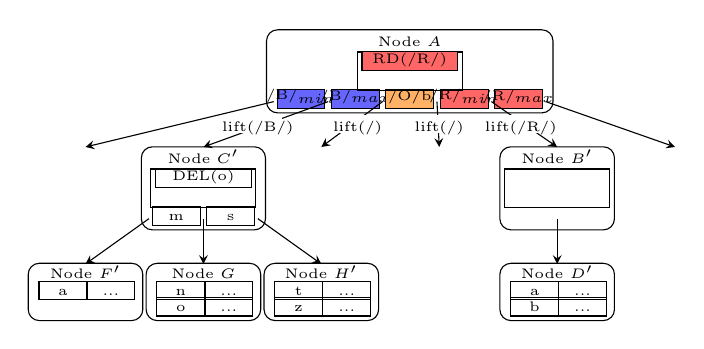
\begin{tikzpicture}[xscale=0.95, yscale=0.95]
            \node[anchor=south, rectangle, rounded corners, minimum height=.06\textwidth, minimum width=.12\textwidth, draw=black] at (-.39\textwidth, 0) {};
            \node[anchor=south, font=\tiny] at (-.39\textwidth, .036\textwidth) {Node $F'$};
            \node[anchor=south, rectangle, minimum height=.015\textwidth, minimum width=.05\textwidth, draw=black] at (-.415\textwidth, .023\textwidth) {};
            \node[anchor=south, font=\tiny] at (-.415\textwidth, .018\textwidth) {a};
            \node[anchor=south, rectangle, minimum height=.015\textwidth, minimum width=.05\textwidth, draw=black] at (-.362\textwidth, .023\textwidth) {};
            \node[anchor=south, font=\tiny] at (-.362\textwidth, .018\textwidth) {...};

            \node[anchor=south, rectangle, rounded corners, minimum height=.06\textwidth, minimum width=.12\textwidth, draw=black] at (-.26\textwidth, 0) {};
            \node[anchor=south, font=\tiny] at (-.26\textwidth, .036\textwidth) {Node $G$};
            \node[anchor=south, rectangle, minimum height=.015\textwidth, minimum width=.05\textwidth, draw=black] at (-.285\textwidth, .005\textwidth) {};
            \node[anchor=south, font=\tiny] at (-.285\textwidth, 0) {o};
            \node[anchor=south, rectangle, minimum height=.015\textwidth, minimum width=.05\textwidth, draw=black] at (-.232\textwidth, .005\textwidth) {};
            \node[anchor=south, font=\tiny] at (-.232\textwidth, 0) {...};
            \node[anchor=south, rectangle, minimum height=.015\textwidth, minimum width=.05\textwidth, draw=black] at (-.285\textwidth, .023\textwidth) {};
            \node[anchor=south, font=\tiny] at (-.285\textwidth, .018\textwidth) {n};
            \node[anchor=south, rectangle, minimum height=.015\textwidth, minimum width=.05\textwidth, draw=black] at (-.232\textwidth, .023\textwidth) {};
            \node[anchor=south, font=\tiny] at (-.232\textwidth, .018\textwidth) {...};

            \node[anchor=south, rectangle, rounded corners, minimum height=.06\textwidth, minimum width=.12\textwidth, draw=black] at (-.13\textwidth, 0) {};
            \node[anchor=south, font=\tiny] at (-.13\textwidth, .036\textwidth) {Node $H'$};
            \node[anchor=south, rectangle, minimum height=.015\textwidth, minimum width=.05\textwidth, draw=black] at (-.155\textwidth, .005\textwidth) {};
            \node[anchor=south, font=\tiny] at (-.155\textwidth, 0) {z};
            \node[anchor=south, rectangle, minimum height=.015\textwidth, minimum width=.05\textwidth, draw=black] at (-.102\textwidth, .005\textwidth) {};
            \node[anchor=south, font=\tiny] at (-.102\textwidth, 0) {...};
            \node[anchor=south, rectangle, minimum height=.015\textwidth, minimum width=.05\textwidth, draw=black] at (-.155\textwidth, .023\textwidth) {};
            \node[anchor=south, font=\tiny] at (-.155\textwidth, .018\textwidth) {t};
            \node[anchor=south, rectangle, minimum height=.015\textwidth, minimum width=.05\textwidth, draw=black] at (-.102\textwidth, .023\textwidth) {};
            \node[anchor=south, font=\tiny] at (-.102\textwidth, .018\textwidth) {...};

            \node[anchor=south, rectangle, rounded corners, minimum height=.06\textwidth, minimum width=.12\textwidth, draw=black] at (.13\textwidth, 0) {};
            \node[anchor=south, font=\tiny] at (.13\textwidth, .036\textwidth) {Node $D'$};
            \node[anchor=south, rectangle, minimum height=.015\textwidth, minimum width=.05\textwidth, draw=black] at (.105\textwidth, .005\textwidth) {};
            \node[anchor=south, font=\tiny] at (.105\textwidth, 0) {b};
            \node[anchor=south, rectangle, minimum height=.015\textwidth, minimum width=.05\textwidth, draw=black] at (.158\textwidth, .005\textwidth) {};
            \node[anchor=south, font=\tiny] at (.158\textwidth, 0) {...};
            \node[anchor=south, rectangle, minimum height=.015\textwidth, minimum width=.05\textwidth, draw=black] at (.105\textwidth, .023\textwidth) {};
            \node[anchor=south, font=\tiny] at (.105\textwidth, .018\textwidth) {a};
            \node[anchor=south, rectangle, minimum height=.015\textwidth, minimum width=.05\textwidth, draw=black] at (.158\textwidth, .023\textwidth) {};
            \node[anchor=south, font=\tiny] at (.158\textwidth, .018\textwidth) {...};

            \node[anchor=south, rectangle, rounded corners, minimum height=.087\textwidth, minimum width=.12\textwidth, draw=black] at (.13\textwidth, .1\textwidth) {};
            \node[anchor=south, font=\tiny] at (.13\textwidth, .163\textwidth) {Node $B'$};
            \node[anchor=south, rectangle, minimum height=.04\textwidth, minimum width=.11\textwidth, draw=black] at (.13\textwidth, .125\textwidth) {};

            \node[anchor=south, rectangle, rounded corners, minimum height=.087\textwidth, minimum width=.13\textwidth, draw=black] at (-.26\textwidth, .1\textwidth) {};
            \node[anchor=south, font=\tiny] at (-.26\textwidth, .163\textwidth) {Node $C'$};
            \node[anchor=south, rectangle, minimum height=.015\textwidth, minimum width=.05\textwidth, draw=black] at (-.29\textwidth, .105\textwidth) {};
            \node[anchor=south, font=\tiny] at (-.29\textwidth, .1\textwidth) {m};
            \node[anchor=south, rectangle, minimum height=.015\textwidth, minimum width=.05\textwidth, draw=black] at (-.23\textwidth, .105\textwidth) {};
            \node[anchor=south, font=\tiny] at (-.23\textwidth, .1\textwidth) {s};
            \node[anchor=south, rectangle, minimum height=.04\textwidth, minimum width=.11\textwidth, draw=black] at (-.26\textwidth, .125\textwidth) {};
            \node[anchor=south, rectangle, minimum height=.015\textwidth, minimum width=.1\textwidth, draw=black] at (-.26\textwidth, .147\textwidth) {};
            \node[anchor=south, font=\tiny] at  (-.26\textwidth, .141\textwidth) {DEL(o)};

            \node[anchor=south, rectangle, rounded corners, minimum height=.087\textwidth, minimum width=.3\textwidth, draw=black] at (-.0325\textwidth, .229\textwidth) {};
            \node[anchor=south, font=\tiny] at (-.0325\textwidth, .292\textwidth) {Node $A$};
            \node[anchor=south, rectangle, minimum height=.015\textwidth, minimum width=.05\textwidth, draw=black, fill={blue!60}] at (-.1525\textwidth, .234\textwidth) {};
            \node[anchor=south, font=\tiny] at (-.1525\textwidth, .229\textwidth) {/B/$_{min}$};
            \node[anchor=south, rectangle, minimum height=.015\textwidth, minimum width=.05\textwidth, draw=black, fill={blue!60}] at (-.0925\textwidth, .234\textwidth) {};
            \node[anchor=south, font=\tiny] at (-.0925\textwidth, .229\textwidth) {/B/$_{max}$};
            \node[anchor=south, rectangle, minimum height=.015\textwidth, minimum width=.05\textwidth, draw=black, fill={orange!60}] at (-.0325\textwidth, .234\textwidth) {};
            \node[anchor=south, font=\tiny] at (-.0325\textwidth, .229\textwidth) {/O/b};
            \node[anchor=south, rectangle, minimum height=.015\textwidth, minimum width=.05\textwidth, draw=black, fill={red!60}] at (.0275\textwidth, .234\textwidth) {};
            \node[anchor=south, font=\tiny] at (.0275\textwidth, .229\textwidth) {/R/$_{min}$};
            \node[anchor=south, rectangle, minimum height=.015\textwidth, minimum width=.05\textwidth, draw=black, fill={red!60}] at (.0875\textwidth, .234\textwidth) {};
            \node[anchor=south, font=\tiny] at (.0875\textwidth, .229\textwidth) {/R/$_{max}$};
            \node[anchor=south, rectangle, minimum height=.04\textwidth, minimum width=.11\textwidth, draw=black] at (-.0325\textwidth, .254\textwidth) {};
            \node[anchor=south, rectangle, minimum height=.015\textwidth, minimum width=.1\textwidth, draw=black, fill={red!60}] at (-.0325\textwidth, .276\textwidth) {};
            \node[anchor=south, font=\tiny] at  (-.0325\textwidth, .27\textwidth) {RD(/R/)};

            \draw[->, >=stealth] (-.32\textwidth, .113\textwidth) -- (-.39\textwidth, .063\textwidth);
            \draw[->, >=stealth] (-.26\textwidth, .113\textwidth) -- (-.26\textwidth, .063\textwidth);
            \draw[->, >=stealth] (-.20\textwidth, .113\textwidth) -- (-.13\textwidth, .063\textwidth);
            \draw[->, >=stealth] (.13\textwidth, .113\textwidth) -- (.13\textwidth, .063\textwidth);
            \draw[->, >=stealth] (-.1825\textwidth, .242\textwidth) -- (-.39\textwidth, .192\textwidth);
            \draw[->, >=stealth] (-.1225\textwidth, .242\textwidth) -- (-.26\textwidth, .192\textwidth);
            \draw[->, >=stealth] (-.0625\textwidth, .242\textwidth) -- (-.13\textwidth, .192\textwidth);
            \draw[->, >=stealth] (-.0025\textwidth, .242\textwidth) -- (0, .192\textwidth);
            \draw[->, >=stealth] (.0575\textwidth, .242\textwidth) -- (.13\textwidth, .192\textwidth);
            \draw[->, >=stealth] (.1175\textwidth, .242\textwidth) -- (.26\textwidth, .192\textwidth);

            \node[anchor=north,rectangle, minimum height=.015\textwidth, minimum width=.05\textwidth, fill={white}] at (-.20\textwidth, .228\textwidth) {};
            \node[anchor=north, font=\tiny] at (-.20\textwidth, .231\textwidth) {lift(/B/)};
            \node[anchor=north,rectangle, minimum height=.015\textwidth, minimum width=.05\textwidth, fill={white}] at (-.09\textwidth, .228\textwidth) {};
            \node[anchor=north, font=\tiny] at (-.09\textwidth, .231\textwidth) {lift(/)};
            \node[anchor=north,rectangle, minimum height=.015\textwidth, minimum width=.05\textwidth, fill={white}] at (0, .228\textwidth) {};
            \node[anchor=north, font=\tiny] at (0, .231\textwidth) {lift(/)};
            \node[anchor=north,rectangle, minimum height=.015\textwidth, minimum width=.05\textwidth, fill={white}] at (.09\textwidth, .228\textwidth) {};
            \node[anchor=north, font=\tiny] at (.09\textwidth, .231\textwidth) {lift(/R/)};
        \end{tikzpicture}
        \caption{\label{subfig:rr-3} The range-rename swaps the subtrees and
            injects a range-delete message for source keys.}
    \end{subfigure}
    \caption[A range-rename example]{\label{fig:rr}
        An example of range-rename(``/R/'', ``/B/'').}
\end{figure}

On lifted \bets, range-rename(\spre, \dpre) can be done with two steps:

\paragraph{Tree Surgery.}
The range-rename first slices out two isolated subtrees in the lifted \bet
simultaneously, one of \spre and the other of \dpre.
The range-rename requires the source and destination subtrees to be at the same
height.
Therefore, for the subtree with a lower LCA, the range-rename keeps slicing its
ancestors by adding nodes with only one child.

\paragraph{Transplant.}
Then, the range-rename swaps these two subtrees and injects a range-delete
message for source key.
Because the source and destination subtree are at the same height, the swap
doesn't violate the \bet invariant that all leaves should be at the same depth.
The range-delete message leverages the existing garbage collection mechanism
to reclaim the destination subtree.

An example of range-rename(``/R/'', ``/B/'') is shown in Figure~\ref{fig:rr}.
Figure~\ref{subfig:rr-1} shows the lifted \bet before the range-rename.
In Figure~\ref{subfig:rr-2}, tree surgery slices out the source subtree, rooted
at Node $C'$, and the destination subtree, root at Node $B'$.
Note though the destination LCA is Node $D$, tree surgery still splits Node $B$
to keep the source and destination subtrees at the same height.
Also, prefix ``/R/'' is lifted from the source subtree and prefix ``/B/''
is lifted from the destination subtree.
Figure~\ref{subfig:rr-3} shows the lifted \bet after swapping the source and
destination subtrees, with a range-delete message for ``/R/'' keys in Node $A$.

\paragraph{Healing.}
The \fti implementation of \bets maintains the invariant that all non-leaf nodes
have between 4 and 16 children, which bounds the height of the tree.
However, tree surgery might break the constraint because it splits nodes with
its own keys.

This situation is handled by triggering a rebalancing within the tree after
the range-rename.
Specifically, if a node has only one child, the slicing process will merge
it after completing the work of the rename.
After the transplant completes, there may be a number of \bet nodes in memory at
the fringe around the source and destination that have fewer children than
desired.
The healing process merges these smaller nodes back together,
using the same approach as a typical \bet merge.
At this point, it is also possible that this could trigger a rebalancing within
the tree.

\paragraph{Complexity.}
During tree surgery, at most 4 root-to-leaf paths are traversed, dirtying all
nodes along the paths.
These nodes will need to be read, if not in cache, and written back to disk as
part of the checkpointing process.
Therefore, the number of I/Os required in tree surgery is at most proportional
to the height of the \bet, which is logarithmic in the size of the tree.

There is also lifting work along all nodes that are sliced in tree surgery or
merged in healing.
However, the number of such nodes is at most proportional to the height of the
tree.
Thus, the number of nodes that must be lifted during a range-rename is no more
than the nodes that must be sliced during tree surgery, and proportional to
the height of the tree.

In summary, the IO cost of a range-rename is $O(log_{B}{N}/\varepsilon)$.

\paragraph{Atomicity and Transactions.}
The \fti in \betrfs implements \bets with multi-version concurrency control by
augmenting messages with a logical timestamp.
Messages updating a given key range are always applied in logical order.
Multiple messages can share a timestamp, giving them transactional semantics.

To ensure atomicity for a range-rename,
read transactions ``before'' the range-rename must complete before the surgery
can proceed.
Each \bet node has a reader-writer lock.
The range-rename write-locks tree nodes hand-over-hand, and left-to-right to
identify the LCAs.
Once the LCAs are locked, this serializes any new read or write transactions
until the range-rename completes.
The lock at the LCA creates a ``barrier''---operations can complete ``above'' or
``below'' this lock in the tree, although the slicing will wait for concurrent
transactions to complete before write-locking that node.
Once the transplant completes, the write-locks on the parents above LCAs are
released.

Briefly speaking, the range-rename ensures all messages representing changes in
the affected key range(s) that logically occurred before the range-rename are
flushed at least to the LCAs.
All messages that logically occur after the range-rename must stay above the
parents of the LCAs.
This strategy ensures that, when each message is flushed and applied, it sees a
point-in-time consistent view of the subtree.

\paragraph{Crash Consistency.}
In general, \fti ensures crash consistency by keeping a redo log of pending
messages and applying messages to nodes copy-on-write.
At periodic intervals, \fti ensures that there is a consistent checkpoint
of the tree on disk.
Crash recovery simply replays the redo log since the last checkpoint.
Range-rename works within this framework.

A range-rename is {\em logically applied} as soon as the
range-rename and its corresponding transaction commit entries are inserted into
the redo log.
The range rename is durable as soon as the redo log entry is written to disk.
If the system crashes after a range rename is logged, the recovery will see a
prefix of the message history that includes the range rename,
and performs the corresponding range-rename on the \bet.

\paragraph{Latency.}
The range-rename returns to the user once a log entry is in the journal and the
root node of the \bet is write-locked.
No other operation on the \bet can proceed before the range-rename releases the
root lock.
The rest of the range-rename work is handed off to background threads, which
performing slicing, transplanting and healing.

\section{Implementation}

\paragraph{\betrfs key order.}
There are 2 constraint on the key order of full-path-index \betrfs with
range-renames:

\begin{itemize}
\item the readdir constraint. Because \betrfs uses range-queries to fetch all
child entries for readdirs, all files and directories immediately under one
directory must be contiguous in keyspace.
\item the lexicographic constraint. Key lifting only works properly with
lexicographic key order. In order to use range-rename, \betrfs must use
lexicographic key order.
\end{itemize}

Simple \texttt{memcmp} key order fails the readdir constraint.
Consider entries ``/bar/dir'', ``/bar/dir/file'' and ``/bar/file'' in the that
order, a readdir for directory ``/bar'' needs to skip ``/bar/dir/file'' in
its range queries.
In the worst case, a readdir might need to skip almost all keys in the key/value
store.

The old \betrfs key order sorts full-path keys first by the number of slashes
and then by a \texttt{memcmp}.
This key order satisfies the readdir constraint but fails the lexicographic
constraint, so \betrfs needs a new key order for range-rename.

In order to adopt range-rename, \betrfs tweaks its full-path keys by adding one
additional slash alongside the last slash.
Now, ``/foo'' and ``/foo/bar'' become ``//foo'' and ``/foo//bar'', respectively
(for correct ordering, `\textbackslash x01' is used as slashes).
With the new full-path keys, \betrfs can use \texttt{memcmp} as the key
comparison function while satisfying the readdir constraint.

\paragraph{Re-lifting nodes.}

\section{Summary}

This chapter presents a new key/value store operation, range-rename.
Renames on full-path-indexed \betrfs can be done with an insert, a delete and
one or two range-renames.
And on lifted \bets, a range-rename can be done efficiently with tree surgery.

\betrfs with range-rename demonstrates the possibility of consolidating
efficient renames into full-path-indexed file systems, showing the possibility
of building file systems that are good at locality and namespace operations.

